\chapter{Late Modern English (1700--1945)}\label{LModE}

\section{History and context}
The period of Late Modern English (LModE) is characterized by notable technological\is{technology} advancements and social changes, which are also reflected in the variation we find in the language of the period. To begin with, Late Modern English saw the introduction of steamships in 1790, railways in 1825, cars in 1763 and 1886,\footnote{Steam-driven in 1763; petrol-driven in 1886.} telephone in 1876, radio\is{media} in 1895, sound-film in 1925, and experimental TV transmission in 1939 \citep[75]{Strang1970}. These technological\is{technology} developments are important for the following reasons. First, they made travelling easier and more accessible and increased dialect contact as a result.\footnote{And of course, over time, this also led to somewhat easier immigration.\is{migration} In case of Britain during the Late Modern English period, this would be primarily immigration associated with former colonies\is{colonialism} of the British Empire.\is{British Empire} Many of these immigrants would not speak English natively.} Secondly, the introduction of the telephone planted the seed of what has by the 21st century become a way to communicate with a potentially large number of individuals living in regions separated by considerable distances on a daily basis. This has again led to more dialect contact. Similarly, the introduction of the radio\is{media} and the TV led to the exposure to those varieties of English that were represented in these media\is{media} at the time, and these varieties of English were -- unsurprisingly -- those that were considered standard.\is{standardization} Due to their representation in these media,\is{media} their ``standardness'' only increased as they became considered the hallmarks of speaking properly in the years to come. 

Communication-related consequences of technology\is{technology} are, however, just one part of the sociolinguistically\is{sociolinguistics} meaningful events of Late Modern English. The industrial revolution,\is{industrial revolution} starting in 1760, impacted society in several ways. Perhaps most importantly, the people in power were no longer just those who had inherited power by birth. The emergence of the nouveau riche (the new rich) had one language-related consequence: although you may have had the wealth and thus also political and social power based on this wealth, your language reflected your social background, that is, at least, unless you consciously or unconsciously changed how you spoke. This created the need to know what the ``correct'' way of speaking was.

In addition to this development, Late Modern English also saw increasing democratization ensuing from the Glorious Revolution (1689), urbanization, and the foundation of the Royal Society, which ``{[}promoted{]} scientific and rational discourse'' \citep[3]{Beal2004}.\is{scientific language} This enlightenment resulted in a ``period ... in which faith was no longer solely placed in an omnipotent God, but in humanity's capacity for rational thinking'' \citep[3]{Beal2004}. These social changes are also important and go hand in hand with the rise of prescriptivism\is{prescriptivism} (see \sectref{prescriptivism}). For instance, some structures began to be perceived as incorrect based on an appeal to ``logic'' or because of comparison to Latin, prime examples being \glossterm{gl-negative-concord}{negative concord}\is{negation} (\textit{\textbf{Ain't}\is{\emph{ain't}} \textbf{no} sunshine when she's gone}), flat adverbs (\textit{\textbf{extreme} unwilling}, \citealp[11]{Mugglestone2003}), and the use of \textit{who} rather than \textit{whom} in sentences such as \textit{those \textbf{who} you love} versus the form traditionally deemed correct, \textit{those \textbf{whom} you love}.

To focus on just one of these constructions, the supposed ``logic'' behind the idea that negative concord\is{negation} is incorrect and indeed formally illogical was the argument that if a sentence contains two negatives (\textit{Ai\textbf{n't no} sunshine}, \textit{I do\textbf{n't} do \textbf{nothing}}), then these two negatives cancel each other out. Thus, \textit{I do\textbf{n't} do \textbf{nothing}} does not mean, according to this argument, that the speaker is not engaging in any activity, but that it is \textit{not} the case that the speaker is not engaging in an activity. This is indeed how negation works in Standard Present Day English, at least in theory. We find similar discussions today surrounding the so-called singular \textit{they}. An example of a singular \textit{they} would be \textit{Everyone should go look for bumblebees if \textbf{they} feel like it}.\is{bumblebees} \citet[273]{Boyd2019} outlines the supposed logic behind the critique of sentences like the bumblebee\is{bumblebees} one containing singular \textit{they} above:

\begin{quote}
    \textit{They} is plural,\is{plurals} so it is ungrammatical to use it with a singular antecedent. The stature of the writer who violates this rule has no bearing on whether the rule is valid, since the logic of the rule is unimpeachable. Shakespeare\ia{Shakespeare, William} does it? ``What a shame,'' says the conservative prescriptivist,\is{prescriptivism} ``I never knew Shakespeare had such bad grammar''.
\end{quote}

\noindent Importantly, arguments based on ``logic'' of the type mentioned above are irrelevant to natural language use. And negative concord\is{negation} in English is very old indeed, since it's the norm as early as the earliest Old English: see \sectref{sec:OE-concord}.

Finally, the technological\is{technology} advancements combined with British colonization\is{colonialism} resulted in the spread of the English language across the globe.\is{globalization} As we saw in \chapref{englishtoday}, most varieties of English as we know it today are only a couple of centuries old, and their establishment as distinct, individual varieties took place during the Late Modern English period. For some, this process is still ongoing. In this chapter, we will focus only on two varieties of English: British English\il{English, British} (and primarily English English) and American English.\il{English, American} Because English came into existence in Britain, we will be discussing English used in Britain during the Late Modern English period. This perhaps somewhat obvious (and admittedly rather traditional) reason is nevertheless not the only motivation to discuss British English and English English in particular. As we will see, what was deemed socially prestigious linguistic behaviour was often related to the norms established in England. We will, however, learn more about the history of American English in this chapter as well. The speakers of American English were some of the first to explicitly and formally rebel against English linguistic norms, and American English\il{English, American} was one of the first and the earliest to see its official recognition as an individual variety of English. In the twentieth century, as we will see particularly in \sectref{LModE-morphology}, the pendulum has swung back in the other direction, and in many contexts American English is socially more prestigious than British English\il{English, British} due to its cultural and technological\is{technology} influence.

In the rest of this section, we concentrate on the rise of prescriptivism,\is{prescriptivism} which characterizes Late Modern English, and its consequences for our understanding of language variation and change\is{language variation and change (field)} not only in Late Modern English but also Present Day English (\sectref{prescriptivism}). The emergence of American English is described in \sectref{LModE-AmE}.\il{English, American}

\subsection{Prescriptivism}\label{prescriptivism}\is{prescriptivism|(}
The word \textit{prescriptivism} originates in the Latin \textit{praescrībere}, meaning literally `to write beforehand' and, more importantly here `to lay down rules, to limit'. In the context of language, prescriptivism is the attempt to establish rules that govern what linguistic usage should or should not be like. Linguistic prescriptivism is something most of us are likely to come across, although not necessarily consciously so. The Accentism\is{accentism} Project by Carrie\ia{Carrie, Erin} \& Drummond\ia{Drummond, Rob} offers a number of examples reported primarily by English speakers,\footnote{\url{https://accentism.org/}.} whether native or non-native. For instance, Sta gives the following story on the Accentism\is{accentism} Project website as someone who is not a native speaker of English (3rd February 2018):

\begin{quote}
    Because I sound so American, it always strikes me when people start correcting my English only after they find out I am not a native speaker and actually from South Asia. Seems I speak it ``like a native'' but only till they figure out my passport. Then it's a giveaway.\is{accentism}
\end{quote}

\noindent Negative attitudes associated with non-native varieties of English fall within the ideology of so-called native-speakerism,\is{native-speakerism} according to which, for instance, only native speakers of English should teach English.\footnote{For an interesting discussion of native-speakerism, see \citet{Jenkins2006} and \citet{FirthWagner1997}.}

Regarding native speakers of English, prescriptivism is typically observable with nonstandard dialects, although it is by no means limited to these. A story by Lisa (28th March 2018) contains a typical example:

\begin{quote}
    When I started at Oxford in the late 80s someone told me, ``You can't possibly be studying English at Oxford with an accent like that!'' This came hot on the heels of a teacher at a study week telling me ``The northern accent is generally associated with being thick.{''}.
\end{quote}

\noindent Prescriptivism is in opposition to descriptivism. A descriptive approach to linguistic variation is one where we describe how speakers use a language, whether they are native or non-native speakers of that language, and whether or not they speak a standard or a nonstandard variety of that language. A prescriptivist approach to variation, however, is a prohibitive one: some types of language-related phenomena are seen as incorrect, and often these correlate with specific social groups. Linguistic research as carried out in academia is descriptive, not prescriptive.

Furthermore, certain properties of language and speech, such as those associated with one's sex and/or gender,\is{gender studies} can also tap into stereotypical biases (e.g. \citealp{Hall1985}). It is very likely that linguistic discrimination of various sorts has been around for as long as any type of discrimination has. When speakers start criticizing the language of others \textit{openly}, however, we are dealing with prescriptivism and proscriptivism: the way one should use language and the way one should not, respectively. We find the first more conventional traces of prescriptivism in the history of English after the language begins to undergo a process of standardization.\is{standardization} This makes sense: after the printing press\is{printing press} was introduced in 1476, a specific variety of English (more in \chapref{EModE}) began to spread in written contexts across the island and, as a result, began to be seen as prestigious (\citealp[9]{Mugglestone2003}; cf. \sectref{EModE-standardization}). Just think of the ``If it's printed, it must be true'' line of thought (see also \citealp[81]{Strang1970}).\is{standardization}

Very indicative of this rise of prescriptivism are the numerous grammar books and dictionaries\is{dictionaries} produced by a range of grammarians of the period.\is{standardization} For instance, an anonymous manual titled \textit{Poor letter H, its use and abuse: addressed to its little vowels,\is{vowels} a, e, i, o, u, and the millions who use them, by the Hon. Henry H.}, published in 1859, was sold in thousands at the time \citep[4]{Mugglestone2003}.\footnote{Some of the authors of these manuals were well known: John Dryden,\ia{Dryden, John} John Hart,\ia{Hart, John} Robert Lowth,\ia{Lowth, Robert} Lindley Murray,\ia{Murray, Lindley} and Richard Mulcaster.\ia{Mulcaster, Richard}}
Thus, we find instruction on the ``best'' language-related practices. Here's an example of an entry from one such manual, the \textit{Critical Pronouncing Dictionary}\is{dictionaries} by John Walker from \citeyear{Walker1823}; this one outlines the desired pronunciation of the word \textit{mercy}: 

\begin{quote}
    The vulgar pronounce this word as if spelled \textit{marcy}, many above the vulgar pronounce it as if written \textit{murcy}; but there is a delicate shade of difference between this and the true sound of \textit{e}, which must be carefully attended to ... \citep[387]{Walker1823}
\end{quote}

\noindent This flourishing of grammar books and instructive materials\is{standardization} clearly shows that audiences of the period were interested in and indeed preoccupied with knowing how to talk properly. This is the beginning of what \citet[249]{Crystal2005} refers to as the complaint tradition,\is{complaint tradition} which has persisted till this day. As Crystal writes, we are indeed dealing with complaining, i.e. focusing on the negatives: ``people do not usually write, phone, or band together to commend usages they like''.  Less direct but still very striking evidence of the general prescriptivism of the period can be frequently found not only in grammar books and manuals, but also in fictional literature of the times, as in the following observation from \textit{Jane Eyre} \citep[444]{Bronte2006}:

\begin{quote}
    She is not an uneducated person, I should think, by her manner of speaking; her accent was quite pure; and the clothes she took off, though splashed and wet, were little worn and fine.
\end{quote}

\noindent In short, there is no lack of evidence from the Late Modern English period that suggests that a concept of ``pure'' English was indeed very much alive.

Resonances of these prescriptive times can be found in the opinion that language change is not good and should be prevented. In the 21st century, language change is frequently seen as language decay (see also Aitchison's \citeyear{Aitchison2012} very accessible and absorbing read titled \textit{Language Change: Progress or Decay?}). We do not have to do too much searching to find judgemental, prescriptive comments like this one \citep{York2017}:

\begin{quote}
    Slang has been around for generations, e.g. ``Swell'' was a popular 1930s approval word, and dozens more descriptive words become trendy but then fade away. Today, however, slang has acquired a new and disturbing quality by ignoring the difference between sexes (guys), grossly overstating (awesome), and adding a different meaning (cool). Much of it is disgustingly vulgar. Worse, it's everywhere and used by people of all ages, backgrounds, educational and economic levels.
\end{quote}

\noindent This perceived decay of the language was also mentioned in \chapref{introduction}. However, systematic study of language variation and change\is{language variation and change (field)} across centuries and a range of languages has shown time and time again that language variation and change are perfectly natural and have taken place for as long as the language in question has been used. That the English language has always been undergoing changes is something we are going to see in the rest of this book.\is{prescriptivism|)}

\begin{figure}
    
\includegraphics[scale=0.34]{chapters/img/bestest.jpg}
    \caption{\textit{best\textbf{est} friends} -- an example of a double superlative; photo taken by Míša in Scotland in 2011}
    \label{fig:bestest}
\end{figure}

\begin{varietybox}{The emergence of Received Pronunciation as a sociolect}
One of the pronunciation standards used in numerous Present Day English dictionaries\is{dictionaries} and textbooks, as well as related audio teaching materials, is \glossterm{gl-RP}{Received Pronunciation},\il{English, Received Pronunciation} often abbreviated just to RP. It is sometimes used interchangeably with BBC English. Where does RP come from?\is{standardization} It is a variety of English based on Standard Southern British (= English!) English.\il{English, Standard Southern British} As \citet{Fennell2001} explains, the term RP ``entered into British common vocabulary'' at the end of the 19th century ``to refer to the educated accent of London and the Home Counties'' \citep[185]{Fennell2001}. It became ``received'' when it had become recognized by speakers as the accent to aim for in order to climb the social ladder. Daniel Jones was the first to call this spoken variety ``Public School English''\il{English, Public School} in 1917. Later in 1926, he termed the same variety of the language Received Pronunciation. Today, RP may have negative connotations\is{accentism} for some -- it can be perceived as too posh, and the characters of evil geniuses (or genii!) are often portrayed with an RP accent in American films (see \citealp{Lippi2012}). The emergence of RP is linked to the establishment of ``public schools'', a small set of private, originally all-male boarding schools traditionally attended by children of the British ruling classes. Public School English, to give rise to RP in time, had a certain type of \glossterm{gl-prestige}{prestige}\is{prestige} attached to it. Interestingly, the mastery of Public School English\il{English, Public School} took on religious associations as well: `In the church, RP\il{English, Received Pronunciation}\is{Christianity} was considered a necessary qualification for Anglicans, whereas ``a non-standard accent in a minister of religion would, until comparatively recently, be a fairly safe indicator that he belonged to a Non-conformist denomination'{''} (\citealp[34]{Honey1989}, in \citealp[61]{Gorlach1999}). 
\end{varietybox}


\subsection{Emergence of American English}\label{LModE-AmE}\il{English, American|(}
In this section, we target varieties of American English spoken in the United States of America. As we saw in \chapref{englishtoday}, American English was certainly seen as a variety in its own right, at least by some Americans, around the years 1775--1783, when the American War of Independence took place. Thus, Noah Webster, an American lexicographer and a spelling reformer, wrote in 1828 that the style of American writers is ``in purity,\is{purism} in elegance and in technical precision, {[}...{]} equaled only by that of the best British authors, and surpassed by that of no English compositions of a similar kind'' \citep[viii]{Webster1828}. He further adds that ``{[}i{]}t is not only important, but, in a degree necessary, that the people of this country, should have an American Dictionary\is{dictionaries} of the English Language; for, although the body of the language is the same as in England, and it is desirable to perpetuate that sameness, yet some differences must exist'' \citep[vi-vii]{Webster1828}. This is a reaction to the fact that in Britain American English was considered ``a tract {[}i.e. trace{]} of corruption'' (Samuel Johnson,\ia{Johnson, Samuel} a prominent English lexicographer, quoted in \citealp[4]{Martin2019}).

Webster was a particularly noteworthy spelling reformer because some of his suggestions have actually caught on -- something most spelling reformers could not boast of. It is thanks to Webster that the word \textit{colour} is spelt as \textit{color} in American English: ``we ought to reject u from honor, favor, candor, error, and others of this class'' (\citealp{Webster1806}, cited in \citealp[435]{ShapiroLynch2017}). He also proposed to unify the spelling of word-final <er> and <re> under <er> (\citealp{Webster1806}, cited in \citealp[434--435]{ShapiroLynch2017}):

\begin{quote}
    The present practice is not only contrary to the general uniformity observable in words of this class, but is inconsistent with itself; for Peter, a proper name, is always written in the English manner. Metre also retains its \ili{French} spelling, while the same word in composition, as in diameter, barometer, and thermometer, is conformed to the English orthography.\is{orthography} Such palpable inconsistencies and preposterous anomalies do no honor to English literature, but very much perplex the student, and offend the man of taste ...
\end{quote}

\noindent American English was, however, not a monolithic entity around the time of the revolution, nor is it today, and nor was it prior to the revolution. To begin with, there have always been various ethnic communities to consider. What probably comes to our mind first are, on the one hand, the original inhabitants of North America and, on the other, the settlers and other types of immigrants.\is{migration} It was not just native speakers of English who came to settle the area that would later become the United States of America. Specific areas of today's US are still associated with influences of -- for instance -- \ili{French} in New Orleans, \ili{German} in Pennsylvania and New York, \ili{Spanish} in Florida, and West African languages in the Lower South \citep[chapter 4]{WolframSchilling-Estes2015}. Other important nationalities in the sociolinguistic\is{sociolinguistics} history of English include native speakers of \ili{Italian}, \ili{Norwegian}, and \ili{Polish}. To give one more specific example, \citet{Herold1997} suggests that the so-called COT-CAUGHT merger,\is{merger} whereby the vowels\is{vowels} in words like \textit{cot} and \textit{caught} become identical, happened in specific regions\is{regional variation} of Pennsylvania due to the influx of native \ili{Polish} speakers in these regions.

In addition to a large number of speakers of languages other than English, there were of course also immigrants\is{migration} from Britain and Ireland. Importantly, these speakers did not speak the same dialect of English, as they came from various parts of those countries. For instance, \citet[104]{WolframSchilling-Estes2015} mention immigrants from Southeastern England coming to Jamestown and ``some two million immigrants\is{migration} of Scots-Irish descent'', who came to America in the 18th-20th centuries. Moreover, ``{[}i{]}t is estimated {[}...{]} that fully one in seven colonists was Scots-Irish {[}by 1776{]}''.\il{English, Scottish}\il{English, Irish}\is{colonialism} It is also important to realize that speakers from Southeastern England were far from speaking a uniform variety of English, and the same goes for speakers of English originating in Ireland and Scotland. Further yet, even those who came from Britain and Ireland were not necessarily native speakers of English, but may rather have been native speakers of \ili{Irish}, Scottish Gaelic,\il{Gaelic, Scottish} and \ili{Welsh}.\footnote{That Celtic languages are indeed fairly different from English can be illustrated by a sentence from \ili{Welsh}: \textit{Beth hoffet ti fwyta?} `What would you like to eat?'. See also \sectref{OE-Celtic} of chapter \ref{OE} for more on Celtic influence in the history of English.} Furthermore, speakers of languages such as Irish, Scottish Gaelic, and Welsh were religious dissenters, unlikely to (aspire to) speak RP.\is{Christianity}

We couldn't possibly present a chapter on Late Modern English in North America without noting the presence of a numerous group of enslaved\is{slavery} individuals brought to North America. Interestingly for the development of African American English, the first generation of enslaved people spoke completely different languages. American history is chequered with struggles for equality, and equality linked to one's ethnicity in particular. The histories of African Americans, the indigenous inhabitants of the Americas (who spoke yet other languages), and other groups in North America present us with ample examples of discrimination. For an example from recent films, see e.g. \textit{The Best of Enemies} by Robin Bissell\ia{Bissell, Robin} from 2019, which depicts discriminatory behaviours towards African Americans. Regarding academic research into linguistic discrimination, the seminal study by \citet{Purnelletal1990} showed -- like other studies focusing on a range of languages and speakers -- that one's accent, such as African American English\il{English, African American} or Chicano English,\il{English, Chicano} can negatively bias the listener.\is{accentism} So, when one of the researchers on the team called landlords using what may be seen as a ``neutral'' (i.e. standard) accent in order to arrange an appointment, he was more likely to succeed than when he adopted an African American English (AAE) accent or a Chicano English\il{English, Chicano} accent. Today, AAE represents one of the traditionally studied varieties of English. It differs from other varieties of English in a range of differences pertaining to all levels of language (see e.g. \citealp{Green2002}, \citealp[Chapter 7]{WolframSchilling-Estes2015}, and the chapters in \citealp{Lanehart2015}).

A considerable amount of ink has been spilt over where AAE\il{English, African American} comes from exactly. \citet[§8.3]{WolframSchilling-Estes2015} review the mainstream hypotheses about the origins of AAE and conclude that we are unlikely to reach a final answer, at least at this stage. The major hypotheses are the Anglicist, the Creolist,\is{creoles} and the Substrate Hypotheses. According to the Anglicist Hypothesis, AAE can be traced back to older stages of English, which it ultimately originates from. According to the Creolist Hypothesis, AAE started off as a pidgin\is{pidgins} and finally became an English-based creole.\is{creoles} Finally, the Substrate Hypothesis argues for a variety of English with an uninterrupted line of descent from other, earlier stages of English, which has nonetheless been influenced by African languages. For much more detail, we refer you to \citet[Chapter 7]{WolframSchilling-Estes2015} and Part 1 of \citet{Lanehart2015}.  

AAE\il{English, African American} nevertheless represents one of \textit{many} ethnolects found in North America today as well as in the past. This is a good reminder that no introductory textbook on the history of the English language can possibly cover all of the variation that exists in the language. However, we hope to pique your interest and steer you in at least some further directions here.\footnote{We also recommend \textit{The hidden treasure of Black ASL: its history and structure}\il{Black American Sign Language} by \citet{McCaskilletal2011}, which comes with a DVD, and the \textit{Talking Black in America} documentary by Walt Wolfram,\ia{Wolfram, Walt} Neal Hutcheson,\ia{Hutcheson, Neal} and Danica Cullinan\ia{Cullinan, Danica} (\url{https://www.talkingblackinamerica.org/}).}\il{English, American|)}


\begin{varietybox}{Languages of the colonizers as languages of the most powerful?}
In the previous chapter, you may have read our pidgin\is{pidgins} and creole\is{creoles} box. If you haven't, we recommend that you do so before engaging with this box. As \citet{SmithKim2019} point out, most of us will think of pidgins and creoles containing linguistic aspects of English (or some other language of the colonizers,\is{colonialism} such as \ili{Dutch} and \ili{French}). It is typically the language of the more powerful group that serves as the main basis for a pidgin. Because of the power dynamic between colonizers and the colonized during British colonization, we might therefore expect English to form the basis of all North American pidgin languages. However, it wasn't always the colonizers who represented the group whose language served as the main basis for a pidgin. Pidgin Delaware\il{Pidgin Delaware} presents an example of a pidgin which originally developed out of contact between the indigenous people of Delaware, North America, whose mother tongue provided the base of the pidgin, and the Dutch colonizers.\is{colonialism}
\end{varietybox}


\noindent Now that we have seen some of the main sociohistorical events relevant for Late Modern English and their consequences for linguistic variation, we can proceed to the specific linguistic phenomena characteristic of this thrilling period in the history of English.

\largerpage
\section{Sounds}
We will first discuss two canonical examples of linguistic variables indicative of the speaker's class which saw rather interesting developments in the period of Late Modern English. The first phenomenon is referred to as /h/-dropping\is{/h/-dropping} and the second as /r/-vocalization.\is{/r/} We will also introduce you to what is known as the FOOT-STRUT split,\is{split}\is{FOOT-STRUT split} which originated in Late Modern English. However, as we will see and as is often the case, the traces of these developments can be found already in the periods preceding Late Modern English. 

\subsection{/h/-dropping: to drop or not to drop?}\label{LModE-hdrop}\is{/h/-dropping|(}
\glossterm{gl-hdrop}{/h/-dropping}\is{consonants|(} refers to when a speaker does not pronounce an /h/ in words historically pronounced with an /h/. When /h/-dropping takes place, words such as \textit{house}, \textit{hill}, and \textit{hum} are pronounced as /aʊs/, /ɪl/, and /ʌm/ rather than /haʊs/, /hɪl/, and /hʌm/. In other words, the /h/ is deleted (or, indeed, dropped). English /h/-dropping is a rather interesting phenomenon, especially if approached from a historical point of view. First, the term is typically used to cover only instances of word-initial /h/-dropping (or /h/-deletion) in lexical words and not grammatical words (\textit{house} vs. \textit{has}), but only if the /h/ is found in a stressed syllable.\footnote{And grammatical words are often unstressed.} This does not mean, however, that we do not come across /h/-deletion in grammatical words, such as \textit{his}, \textit{him}, and \textit{her}.\footnote{If you ever wondered where the English \textit{'em} comes from, as in \textit{Track 'em, find 'em, kill 'em} from the film \emph{Expendables 2} (2012), it does not come from \textit{them} but an older pronoun\is{pronouns} used for the third person plural:\is{plurals} \textit{hem} (more in \sectref{ME-pronouns} on \textit{them} and \textit{hem}). \textit{Hem} [hɛm] changed to [ɛm] $\sim$ [əm], which gives us the spelling variant <'em>.} As we will see in \chapref{ME}, dropping one's /h/s in grammatical words is a fairly old phenomenon. In Present Day English all English speakers are bound to drop their /h/s in grammatical words. Grammatical words are well-known for such reductions:\is{vowel reduction} for example, the preposition \textit{to} is frequently\is{frequency} reduced to {[}tə{]} or even just {[}t{]}. /h/-deletion in grammatical words therefore shouldn't come as a surprise -- it's just one of the many possible reductions relevant for grammatical words. So now we know that the phenomenon called /h/-dropping, at least in the history of English, typically refers to word-initial deletion of /h/ in the stressed syllables of lexical words.\footnote{However, \citet[157]{Beal2004}, for instance, uses /h/-dropping to also cover the merger\is{merger} of /w/ and /ʍ/, resulting in \textit{Wales} and \textit{whales} sounding alike. See Chapters \ref{introduction} and \ref{ME} for more details.}

There is nevertheless a rather important difference between /h/-deletion related to lexical as opposed to grammatical words. Deleting one's /h/s in grammatical words goes pretty much unnoticed (e.g. \citealp[56]{Barber1964}). On the other hand, /h/-deletion in lexical words, or in stressed grammatical words, is stigmatized. So, in an article on Tony Blair's\ia{Blair, Tony} pronunciation, a commentary raises the following questions: ``But joking aside, where were the Prime Minister's T's? What happened to his H's?'' \citep{Lyall1998}.

\largerpage
Dropping one's /h/s was heavily stigmatized in Late Modern English. We can find instances of /h/-dropping in the earlier periods (as we shall see in \sectref{ME-hdrop} of \chapref{ME}), but it is in Late Modern English that /h/-dropping becomes one of the hallmarks of perceived pronunciation inadequacy. We have already seen that a manual existed devoted solely to the \textit{Poor letter H: its use and abuse}, for dropping one's /h/s could be seen as social suicide (!) at the time \citep[4]{Mugglestone2003}. \citet[159]{Beal2004} dates the stigmatization of word-initial /h/-dropping to the latter half of the 18th century, which is in line with \citet[81]{Strang1970}.

As we go back in time, however, we need to make the discussion a little bit more nuanced. The words mentioned above, \textit{house}, \textit{hill}, and \textit{hum}, are all of Germanic origin. In other words, they have been part of the English language since its emergence. As we will discuss in detail in \chapref{ME}, the period of Middle English (1150--1500) saw a great influx of words of \ili{French} origin. Present Day French words spelt with <h>, as in \textit{honneur} `honour' and \textit{hommage} `homage', do not reflect the fact that there is no /h/ in the pronunciation -- as is also the case in the English equivalents, all loans\is{borrowings} from French. Importantly, in words of French origin, it was desirable not to pronounce the /h/ as written, as this was what was done in French pronunciation, and French was socially prestigious. By the time of Late Modern English, this may have led to confusion if you did not speak French and/or if you did not use words of \ili{French} origin, especially those typically associated with learned vocabulary as well. It was also -- if not primarily -- because of this that manuals and dictionaries\is{dictionaries} for native speakers were available at the time, in which users could consult whether or not a specific word should be pronounced with an /h/. Some such examples are for instance Walker's \textit{Walker remodelled: a new critical pronouncing dictionary}\is{dictionaries} and James Elphinston's\ia{Elphinston, James} \textit{Principles of the English language digested: or, English grammar reduced to analogy.\is{analogy} In Two Volumes}.\footnote{But see \citet{Feddema2013}, who disagrees with the theory that /h/-dropping may have been due to contact with French.}

\largerpage[2]
Over time, some words that had historically no /h/ nevertheless acquired an /h/ in standard English, such as \textit{herb}, from the Old French\il{French, Old} \textit{erbe}.\footnote{The Present Day French form is \textit{herbe}.} Interestingly, whilst in American English\il{English, American} the typical pronunciation is the more conservative /h/-less one, {[}ɜːɹb{]}, what we find in standard British English\il{English, British} is the more innovative version containing an /h/, {[}hɜːb{]}. Other words originally lacking an /h/ include \textit{hospital}, \textit{hotel}, and \textit{humble} \citep[145, 148]{Mugglestone2003}. In some cases, there is still variation within a single regional variety,\is{regional variation} as in the case of \textit{historic} {[}hɪstɒɹɪk{]} $\sim$ {[}ɪstɒɹɪk{]}. 

The phenomenon of /h/-dropping enables us to introduce the concept of \textsc{hypercorrection}.\is{hypercorrection} If you are someone who drops their /h/s, as in words such as \textit{harm} [ɑːm], and you live in a society in which such /h/-dropping is stigmatized, you might start doing your best to make sure that you do not drop your /h/s as that affords you certain social benefits. However, this might pose certain challenges. In the pronunciation of a regular /h/-dropper, words such as \textit{harm} and \textit{arm} sound the same. If you then attempt to avoid /h/-dropping as someone who can't necessarily tell which words do or do not have a historical /h/, you might overdo it by introducing the /h/ also in words that historically do not have this phoneme, as in \textit{arm} [hɑːm]. In hypercorrection, then, the prestigious variant is overused rather than underused. Thus, /h/-dropping-related hypercorrection manifests itself by inserting /h/s in new contexts because it's better to be safe than sorry. Hypercorrection\is{hypercorrection} is nevertheless by no means limited to /h/-dropping!


\begin{soundbox}{Even Latin speakers /h/-dropped}
\ili{Latin} was often viewed as the language to look up to. Interestingly, however, \citet[106]{Minkova2014} mentions an example of \glossterm{gl-hdrop}{/h/-dropping} in Latin texts written by \iai{Saint Augustine}, from the period 354--430. Even Latin speakers /h/-dropped! Would this make the prescriptivists\is{prescriptivism} turn in their graves, we wonder?\is{/h/-dropping|)}
\end{soundbox}


\subsection{/r/}\label{LModE-r}\is{rhoticity|(}
One of the features that distinguishes most British and American English\il{English, British}\il{English, American} accents is \textsc{rhoticity} {[}ɹəʊˈtɪsɪtɪ{]}. Accents can be rhotic ({[}ɹəʊtɪk{]} $\sim$ {[}ɹɒtɪk{]}), non-rhotic, or somewhere in between. What does it mean for an accent to be rhotic or non-rhotic? If you speak with a rhotic accent, any time you see an <r> in the orthographic\is{orthography} representation of a word, you indeed also have an /r/ of some sort in your pronunciation of that word. However, this is not the case for non-rhotic speakers. Thus, if we think of words with a postvocalic /r/, such as \textit{car}, \textit{cart}, \textit{card}, \textit{far}, and \textit{fart}, the transcription relevant for accents such as Standard Southern British English\il{English, Standard Southern British} would simply ignore the /r/s implied by the orthography,\is{orthography} because SSBE speakers do not have these postvocalic /r/s in their accents: /kɑː/, /kɑːt/, /kɑːd/, /fɑː/, /fɑːt/.

Although Present Day American English\il{English, American} is generally known as rhotic and British English\il{English, British} as non-rhotic, the situation is not that straightforward. In today's British English, Scottish English\il{English, Scottish} is rhotic, as is the English we find in Northern Ireland.\il{English, Northern Ireland} Welsh English\il{English, Welsh} and English English, on the other hand, are known as non-rhotic. But even this is simplistic. We do find certain regions in England associated with rhotic accents, such as some parts of Cornwall and Blackburn.\is{regional variation} Similarly, some speakers of Welsh English may pronounce postvocalic /r/s as a result of their L1, since all <r>s are pronounced as such in \ili{Welsh}. Finally, Scottish English\il{English, Scottish} has been recently reported to be losing its postvocalic /r/s in certain regions\is{regional variation} and strata of the society \citep{StuartSmith2013}.

Not surprisingly, American English\il{English, American} also presents us with variation in terms of rhoticity. New York English\il{English, New York} has been traditionally known for being non-rhotic (see what Woody Allen\ia{Allen, Woody} does, for example, in Exercise \ref{exercise-r}), although this has been changing in the course of the 20th and the 21st centuries \citep{Becker2014}, with rhoticity becoming more and more established. Boston\il{English, Boston} is another area traditionally associated with non-rhoticity. However, similarly to NY English, rhoticity has also been making inroads in this variety and increasing in frequency\is{frequency} \citep{Nagy2010}. Such changes from a primarily non-rhotic to a rhotic variety might present us with interesting cases of hypercorrection.\is{hypercorrection} Figure \ref{fig:sourvenirs} shows a spelling\is{orthography} of the word \textit{souvenir} which contains an <r> (<sourvenir>), which is very suggestive of the author overusing postvocalic /r/s, and thus of hypercorrection.\is{hypercorrection} Finally (for the purposes of this chapter), non-rhoticity is one of the phonological features associated with AAE\il{English, African American} (e.g. \citealp{Becker2014} and \citealp{Thomas2007}). The non-rhoticity of AAE is rather interesting in that we can also find the absence of /r/ intervocalically, as in [flɑəɾə] for \textit{Florida} \citep[454]{Thomas2007}. 


\begin{figure}
    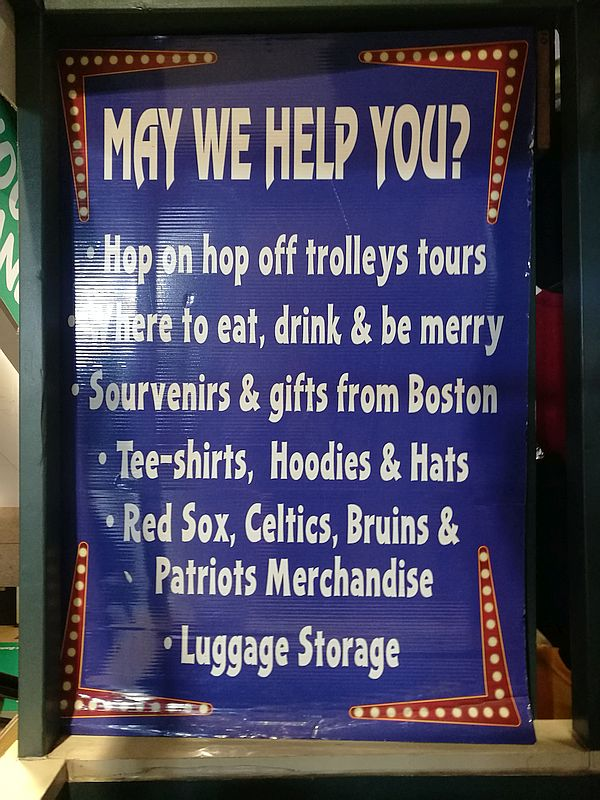
\includegraphics[scale=0.55]{chapters/img/sourvenirs.jpg}
    \caption{\textit{sou\textbf{r}venirs} in Boston, Massachusetts, US; photo taken by our colleague Kamil Kaźmierski in 2019}
    \label{fig:sourvenirs}
\end{figure}

\newpage
To sum up, rhoticity is more complex than a simple division between rhotic and non-rhotic accents. First, we find variation within specific varieties, and secondly even speakers from the same region can show variation.\is{regional variation} Even single individuals can be sometimes rhotic and sometimes non-rhotic, depending on a range of social and language-internal factors (see \citet{Becker2014} for a nice overview of the relevant social constraints).\footnote{As you may know by now from your English phonetics and phonology classes, we also find plenty of variation in how those /r/s that are pronounced by English speakers are realized phonetically. We find a plethora of variants, including a voiced approximant {[}ɹ{]}, a labio-dental approximant {[}ʋ{]}, a retroflex approximant {[}ɻ{]}, an alveolar trill {[}r{]}, and a uvular fricative {[}ʁ{]}. If interested in Present Day English /r/s, see \citet{Wells1982b}. We will revisit this issue briefly in \chapref{OE}.}

Where does all this variation come from? And why have we just spent so much space discussing Present Day English variation in rhoticity in a chapter on Late Modern English? As you may have just guessed, it is the Late Modern English period which -- to an extent -- holds the key to our understanding of just what has happened to English /r/ and the reasons for its current state in Present Day English. Similarly to /h/-dropping,\is{/h/-dropping} Late Modern English speakers first started vocalizing just some of their /r/s. When American English\il{English, American} was being established as a variety of English, English in Britain, the island of Ireland, and North America was a rhotic English. This started changing in England, where postvocalic /r/ first began to weaken to a schwa /ʃwɑː/. It could be, and ultimately was, deleted altogether in many (though not all) accents. 

Certain communities in North America were looking up to Britain, and tended to adopt Britain-oriented norms. As a result, non-rhoticity was the prestigious norm in these communities, which lasted variably throughout the 20th century \citep[142]{Becker2014}. However, some of the earliest studies that investigated the use of this variable highlighted the complexity of the situation and the extent to which standard language is an arbitrary concept.\is{standardization} \citet{Labov1966} showed that postvocalic /r/ in New York English,\il{English, New York} a traditionally non-rhotic variety, was associated with prestige\is{prestige} at the time of his study. This contrasts with the prestige\is{prestige} that non-rhoticity had in NY earlier, and it also contrasts with areas such as Charleston, where the absence of /r/ was also seen as prestigious originally.\footnote{Similarly to what Labov has shown for NY English, \citet[Chapter 4]{Baranowski2006} shows that rhoticity has won the day in Charleston as well.}\il{English, Charleston} In a nutshell, what we end up with is roughly this: in NY it was rhoticity that ended up being seen as prestigious, whereas it was the opposite, non-rhoticity, which had been established as the norm to aspire to in English English \citep[139]{Montgomery2001}.

This is somewhat ironic, considering that /r/-lessness was stigmatized when it made its first appearance in England: ``[m]any writers (and speakers) [...] seemed to cultivate an ostrich-like mentality, resolutely refusing to acknowledge that such a change had taken place, or that, if it had, it had done so only in the most vulgar of surroundings'' \citep[99]{Mugglestone2003}. When the weakening of /r/ was first noticed in English in the 18th century, it was commented on negatively:\is{accentism}

\begin{quote}
    But if this letter {[}i.e. the letter <r>{]} is too forcibly pronounced in Ireland, it is often too feebly pronounced in England, and particularly in London, where it is sometimes entirely sunk. (Walker 1791: 51, in \citealp[153]{Beal2004})\ia{Walker, John}
\end{quote}

\begin{quote}
    It was stigmas of this sort which were used to hound Keats,\ia{Keats, John} whose rhymes of \textit{thorns}/\textit{fawns}, and \textit{thoughts}/\textit{sorts} contravened popular notions of correctness [...], even if they did agree with the realities of linguistic usage at the time. Keats's use of aural rather than visual authority in his poetry\is{poetry} was, however, typically to bring censure rather than praise. \citep[101--102]{Mugglestone2003}
\end{quote}

\noindent \citet[154]{Beal2004} provides contemporary evidence of manuals on ‘good' pronunciation of the times that points to a continuing stigmatization of /r/-vocalization also ``throughout most of the nineteenth century''. As said earlier, changes of this type are often dormant in a language, and this was also the case with post-vocalic /r/.\footnote{See \citet{Minkova2014} for some early examples attested already in Old English (600--1150).}


\begin{soundbox}{Linking and intrusive /r/}
We need to at least touch upon two phenomena related to /r/, which are relevant only for non-rhotic varieties of English and whose origin is tied to that of the origin of non-rhoticity. The first is known as \textsc{linking /r/} and the second as \textsc{intrusive /r/}. Linking /r/ is not stigmatized and refers to when postvocalic /r/s are pronounced despite the accent's usual non-rhoticity. These linking /r/s are pronounced when a postvocalic /r/, as in \textit{car}, is followed by another vowel,\is{vowels} which is part of the following word, as in \textit{The car I like.} {[}ðəˈkɑː\textbf{ɹ}aɪˈlaɪk{]}. Intrusive /r/, on the other hand, is stigmatized {\citep[127]{Minkova2014}}: in Present Day English, it is to a large extent through the knowledge of how English words are supposed to be spelt that speakers can know whether there is an underlying /r/ which can resurface as a linking /r/. However, speakers do not have historical memories that go beyond their own lifespan. This sometimes results in inserting a ``linking'' /r/ where this ``linking'' /r/ has no business to be, so to speak. The most famous instance of this intrusive /r/ can be seen in the pronunciation of \textit{Law and Order} as {[}lɔːɹənɔːdə{]} -- as we can see, the spelling\is{orthography} does not suggest that there has ever been an /r/ in \textit{law} historically, which is indeed the case. Intrusive /r/ is another example of hypercorrection.\is{hypercorrection}\is{consonants|)}\is{rhoticity|)}
\end{soundbox}


\noindent So far, we've focused on two consonantal\is{consonants} features very relevant for Late Modern English, as well as Present Day English. The last phonological feature we will focus on, the so-called FOOT-STRUT split,\is{split} is related to the \textsc{vowel}\is{vowels} system of English.

\subsection{FOOT-STRUT split}\is{vowels|(}\is{split|(}\is{FOOT-STRUT split|(}
An important phonological change that took place in Late Modern English is the FOOT-STRUT split. But first of all, what is a split? A split refers to the process whereby a language acquires a new \glossterm{gl-phoneme}{phoneme} (phoneme B), which develops from an already existing phoneme (phoneme A). However, it is not the case that the phonetic realization of phoneme A simply changes to another realization, realization B (as in {[}A{]} > {[}B{]}). In the new situation, we get the new B, but we still get the older A, thus /A/ > /A/ as well as /B/, and /A/ and /B/ are contrastive. In standard varieties of English, the words \textit{foot} and \textit{strut} are pronounced with two different phonemes: e.g. /fʊt/ and /stɹʌt/. That the vowels /ʊ/ and /ʌ/ are indeed two phonemes is nevertheless more visible if we compare words such as \textit{put} /pʊt/ and \textit{putt} /pʌt/, \textit{look} /lʊk/ and \textit{luck} /lʌk/, or \textit{book} /bʊk/ and \textit{buck} /bʌk/. If we replace one with the other, we get a different word, not just a phonetic variant of the same word.

Before the FOOT-STRUT split happened, the words that now contain the /ʌ/ phoneme, as in \textit{strut} (STRUT), used to have the same phoneme as words such as \textit{foot} (FOOT). Words such as FOOT used to have an /oː/ vowel (/foːt/), which -- as we will see in \chapref{EModE} -- underwent a change to /uː/ in Early Modern English (/fuːt/). In Late Modern English, this vowel was then shortened\is{vowel shortening} and laxed into an /ʊ/ (/fʊt/). Words such as STRUT, until Late Modern English, did not experience quite that much vocalic excitement: the STRUT vowel remained phonologically stable and reflected an /u $\sim$ ʊ/. Thus, by the time of Late Modern English, FOOT and STRUT came to contain the same vowel phoneme: /u $\sim$ ʊ/. However, although this change is reflected in most varieties of English, there are still accents in which we find the pre-split situation. Northern England\il{English, Northern England} varieties typically show FOOT and STRUT with the same vowel phoneme category, /ʊ/ (see for instance \citealp{BaranowskiTurton2018} or \citealp{Strycharczuketal2019}), and these two words therefore rhyme in the varieties in question (e.g. /fʊt/ and /strʊt/). This is also the case for some Irish accents,\il{English, Irish} such as that spoken in Dublin \citep[422]{Wells1982b}.


\begin{soundbox}{The social life of STRUT}
The exact phonetic relation of STRUT is subject to variation in Present Day English varieties.\is{regional variation} For example, even in the north of England, there are speakers who do have two vowel categories for FOOT and STRUT, but they may reflect a vowel quality in STRUT somewhere in between that of FOOT (/ʊ/) and that of the Standard Southern British English\il{English, Standard Southern British} (SSBE) /ʌ/ (\citealp[111]{ChambersTrudgill1998}, and also \citealp{BaranowskiTurton2018}). Irish accents have been noted to have a more centralized quality of STRUT than SSBE and RP \citep[421]{Wells1982b}. Interestingly, Irish English\il{English, Irish} and Northern England English\il{English, Northern England} are not the only varieties of English that differ in their phonetic realization of STRUT from RP and SSBE. Welsh English\il{English, Welsh} tends to show a [ə] in the STRUT words (\citealp{Hejna2018}; \citealp[383]{Wells1982b}). And things definitely do not end here as regards the phonetic and phonological variation of STRUT.\is{vowels|)}\is{split|)}\is{FOOT-STRUT split|)}
\end{soundbox}

\section{Morphology}\label{LModE-morphology}
Language change, especially if related to the structural properties of a language rather than for example newly coined lexical items, has been said to show ``long stretches of dormancy'' \citep[96]{Strang1970}. What this means is that, very frequently, seeds of a change can be found in the language centuries before the change becomes particularly noticeable: it often takes centuries for changes to complete. That this is indeed the case is something we will see repeatedly in the remainder of this book. In this particular section, however, we focus on negative contraction\is{negation} and the history of what is known as the subjunctive.\is{subjunctive} Both of the changes discussed have drawn hostile comments from prescriptivists\is{prescriptivism} over the years.

\subsection{Negative contraction}\label{LME-contraction}\is{inflection|(}\is{negation|(}\is{clitics|(}\is{affixes|(}
In the sentence \textit{You \textbf{shouldn't} do that!}, do you think that \textit{shouldn't} is one word or two? Decide what you think before reading further. Don't base your answer just on the spelling -- that's only one part of the story.

The answer you have arrived at probably depends on what you think the status of the Present Day English negative \glossterm{gl-morpheme}{morpheme} -\textit{n't} is. Under one view, -\textit{n't} is an \glossterm{gl-inflection}{inflectional} suffix, part of the single word \textit{shouldn't} -- and therefore belongs to the domain of (inflectional) morphology.\footnote{For the distinction between inflectional morphology and word-formation, see \sectref{morphology}.} Under the other view, -\textit{n't} is a \glossterm{gl-clitic}{clitic}, a form of the word \textit{not} that just happens to be phonologically reduced and attached to the end of the modal\is{modals} \textit{should} -- and therefore we're really dealing with two separate syntactic words here, \textit{should not}.

In this book we deal with syntax and morphology in separate sections of each chapter. However, in real life, the boundary between syntax and morphology is not always that clear. The morpheme -\textit{n't} is one such case, and part of the fun of linguistics is to look beyond the surface in order to figure out what's really going on in cases like these. The use of -\textit{n't} rather than \textit{not} is usually called \textsc{negative contraction}. Linguists have developed a range of tests to figure out whether elements like -\textit{n't} are inflectional affixes or clitics. The traditional view (e.g. \citealp{Zwicky1969}) is that -\textit{n't} is a clitic. \citet{ZwickyPullum1983}, however, look in depth at this morpheme, apply the linguistic tests, and come to the conclusion that it is in fact an inflectional suffix.

One test pointing in this direction (among many) is the fact that the base to which -\textit{n't} attaches displays some pretty weird behaviour. It's easy to see how you can get from \textit{should} to \textit{should\textbf{n't}}: a simple rule of ``add -\textit{n't}'' will do the trick. But what about \textit{will} and \textit{wo\textbf{n't}}? Here you can't simply ``add -\textit{n't}'', because that would give you the ungrammatical form *\textit{will\textbf{n't}}. But there's no word *\textit{wo} meaning `will', either. So we're forced to treat \textit{will} and \textit{wo\textbf{n't}} as two different inflectional forms of the same word.\footnote{We can make the same argument using \textit{do} and \textit{do\textbf{n't}}, though this time it's not obvious from the spelling. Remember, letters are not sounds -- see \sectref{phonphon}! In British English,\il{English, British} these are pronounced {[}duː{]} and {[}dəʊnt{]} respectively (American English\il{English, American} {[}duː{]} and {[}doʊnt{]}). This is not what you'd expect from simply sticking {[}duː{]} and {[}nt{]} together.} \citeauthor{ZwickyPullum1983}'s paper contains several other arguments all pointing in the same direction: Present Day English -\textit{n't} is an affix, not a clitic.

The forms with -\textit{n't} are found only with the auxiliaries:\is{auxiliaries} \emph{have}, \emph{be}, \emph{do} and the modals\is{modals} (on which see \sectref{EModE-do}). They're not possible with ordinary lexical verbs: *\textit{play\textbf{n't}}, *\textit{eat\textbf{n't}}, *\textit{goes\textbf{n't}}, for instance, are not found. The -\textit{n't} forms rose to prominence during the Late Modern English period, as shown in Figure \ref{fig:NegCont}. This figure is based on the \glossterm{gl-corpus}{Corpus}\is{corpora} of Late Modern English Texts \citep{CLMET3}, which contains texts by British authors from between 1710 and 1920 split into three 70-year periods.\footnote{This figure is inspired by, and replicates findings presented in, \citet{Nakamura2012}, using a different data source.} Initially, we can see that \textit{don't} is far ahead of all the other contractions, but by the final period other contractions are catching up. Of course, we have to be careful with this evidence, as \glossterm{gl-standardization}{standardization}\is{standardization} and prescriptivism\is{prescriptivism} probably meant that the innovative spelling\is{orthography} -\textit{n't} lagged far behind contraction in speech in terms of rate of use.

\begin{figure}[t]
    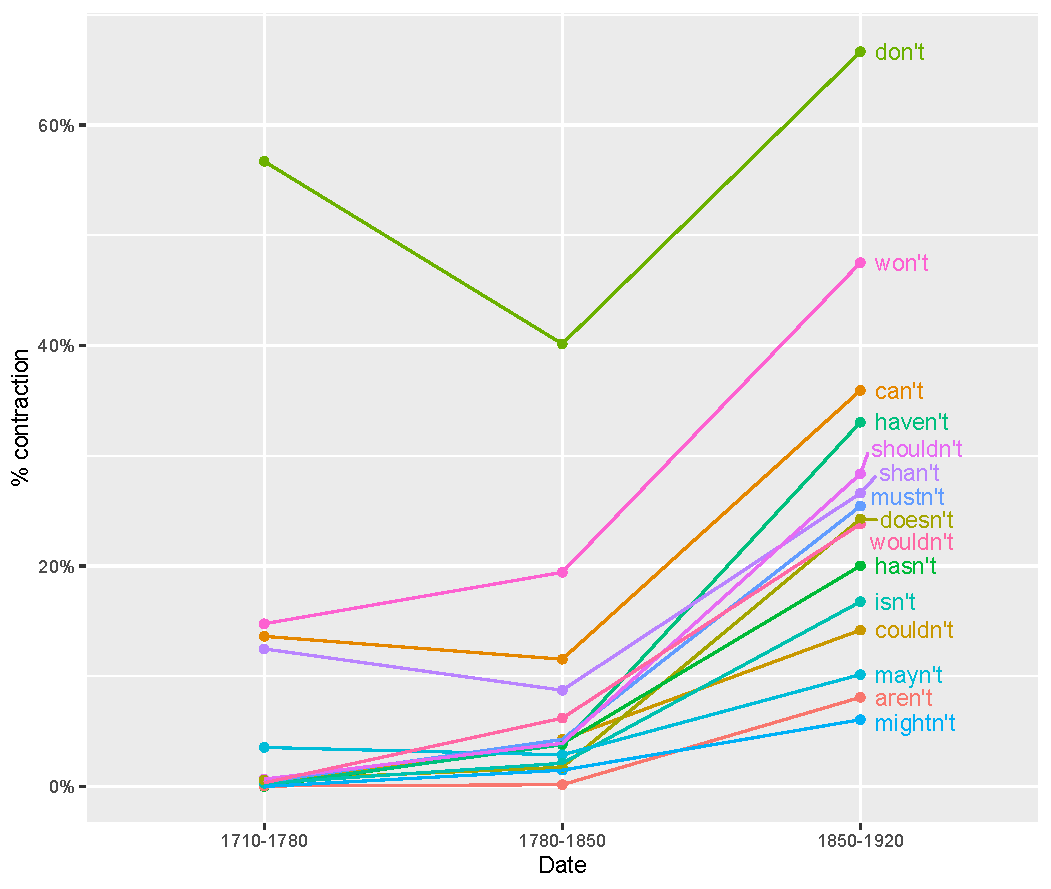
\includegraphics[scale=0.7]{chapters/img/neg-contraction.pdf}
    \caption{Negative contraction as a proportion of use (e.g. \textit{should not} vs. \textit{shouldn't}) during the Late Modern English period. Data from CLMET 3 \citep{CLMET3}.}
    \label{fig:NegCont}
\end{figure}

The data shown in Figure \ref{fig:NegCont} suggests that -\textit{n't} probably wasn't always an inflectional suffix. During the period 1710--1780, we see that the only contractions that occur more than five percent of the time were the ones whose stem ended in a vowel,\is{vowels} a nasal or a liquid (\textit{do}, \textit{will}, \textit{can}, \textit{shall}), with other contractions virtually nonexistent. This apparent phonological conditioning suggests that in this early period we're dealing with a clitic after all, which only later became an affix. Clitics becoming affixes is a common pathway of language change cross-linguistically: it's part of a process called \glossterm{gl-grammaticalization}{grammaticalization}\is{grammaticalization} (see \sectref{linguistic-interaction}), and changes in which two separate words become a single word are referred to as \glossterm{gl-univerbation}{univerbation}. We'll see several more examples of this kind of change throughout the book.\is{clitics|)}\is{affixes|)}


\begin{miscbox}{\textit{Ain't}}
The\is{\emph{ain't}} negative contraction \textit{ai\textbf{n't}} -- as in \textit{If it \textbf{ain't} broke, don't fix it} -- remains one of the most stigmatized words in the English language as far as prescriptivists\is{prescriptivism} are concerned, even though it is found in almost every known variety of English \citep[311--316]{Anderwald2012}. It's exceptionally prevalent in American English,\il{English, American} but also found to a great extent in traditional British English\il{English, British} dialects, and to a lesser extent in varieties of English elsewhere (e.g. New Zealand).\il{English, New Zealand} Needless to say, there's nothing logically or aesthetically wrong with it. \textit{Ain't} can mostly be used as a negated form of \emph{BE} or \emph{HAVE}. Especially in African American English,\il{English, African American} it also replaces \textit{didn't}, as in \textit{I \textbf{ain't} shut my eyes last night} \citep{Howe1997}. Like other negative contractions, \textit{ain't} really gained ground during the Late Modern English period. You can find out more about \textit{ain't} in the papers in \citet{DonaherKatz2015}. And if you wonder where it comes from, let's just say it belongs to the same historical stem as Present Day English \textit{am}.\is{negation|)}
\end{miscbox}


\subsection{The ``subjunctive''}\label{LModE-subjunctive}\is{subjunctive|(}

Take a look at the following sentences of Present Day English:

\begin{exe}
\ex It is important that he \textbf{leave}.\label{exsubjunctive}
\ex It is important that he \textbf{leaves}.\label{exindicative}
\ex It is important that he \textbf{should leave}.\label{exmodal}
\end{exe}

\noindent All three sentences mean roughly the same thing, but the form of the verb is different. In example (\ref{exsubjunctive}) there is no third person singular ending on the verb \textit{leave}, unlike in (\ref{exindicative}). Meanwhile, in (\ref{exmodal}) there's a modal,\is{modals} \textit{should}.

Sentences like (\ref{exsubjunctive}) are sometimes said to contain a morphological \glossterm{gl-subjunctive}{subjunctive}, but this is misleading. The term ``subjunctive'' has its origins in the traditional grammar of classical languages like \ili{Latin} and \ili{Greek}. In languages like these, verbs have special morphological forms -- \glossterm{gl-inflection}{inflections} -- that indicate the speaker's attitude to what they are saying. This is called \glossterm{gl-mood}{mood}, and moods commonly found in European languages include the indicative, the subjunctive and the imperative. Generally, in these languages the subjunctive is used to express \textsc{irrealis} meaning: the speaker is not committing themselves to the truth of the statement. In \ili{German}, for example, the usual third person singular form of the verb \textit{sein} `be' is \textit{ist} `is', but the special subjunctive form is \textit{sei}. The form \textit{ist} is \glossterm{gl-indicative}{indicative}, which is the normal mood used most of the time without any special meaning.

Unlike \ili{Greek}, \ili{Latin}, \ili{French} or \ili{German}, English doesn't have any special morphological forms for mood, including the subjunctive. Instead, ``subjunctive'' sentences like (\ref{exsubjunctive}) just contain the default form of the verb -- it's always the same as the verb's infinitive form. This is made clear when we look at examples (\ref{besubjunctive})--(\ref{bemodal}), containing forms of \emph{BE}.

\begin{exe}
\ex It is important that he \textbf{be} good.\label{besubjunctive}
\ex It is important that he \textbf{is} good.\label{beindicative}
\ex It is important that he \textbf{should be} good.\label{bemodal}
\end{exe}

\noindent Example (\ref{besubjunctive}) contains the non-finite form \textit{be}. That is, since English doesn't have any distinct morphological subjunctive inflection, it doesn't make much sense to say that English has a subjunctive under the traditional, morphological interpretation of the term.\footnote{It's possible, of course, to argue that English \textit{does} have a morphological subjunctive, and that its forms just happen to be written and pronounced in exactly the same way as the infinitive. But this is a pretty weird way of thinking, and is motivated only by the desire to shoehorn the English language into grammatical categories that were developed for \ili{Latin} and \ili{Greek}. Perhaps a better way of thinking about it is provided by \citet[40--42]{Roberts1985}: clauses like (\ref{exsubjunctive}) and (\ref{besubjunctive}) contain a modal\is{modals} which is unpronounced. This accounts for the fact that such clauses behave like other finite clauses while the verb form itself appears to be non-finite.} Does it make sense to say that Present Day English has a subjunctive at all, then? In the \textit{Cambridge grammar of the English language}, \citet[88]{HuddlestonePullum2002} make it clear that they use the term ``subjunctive'' for a syntactic construction, and not for a morphological mood (see also \citealp{Aarts2011}).\is{inflection|)} What \citet{HuddlestonePullum2002} call the subjunctive construction is found exclusively in finite embedded clauses.\footnote{Apart from a few fixed phrases, such as \textit{Long live the king!}. \citet[87]{HuddlestonePullum2002} argue that ``irrealis \textit{were}'', as in \textit{If I \textbf{were} you}, is a different phenomenon, not part of the subjunctive construction; see their book for details.} Other linguists prefer to abolish the term entirely in English grammar \citep{Palmer1988}. This option is tempting, as there are few things that annoy prescriptivists\is{prescriptivism} more than telling them that English doesn't have a subjunctive! In the rest of this book, though, we'll use the term \textsc{subjunctive construction}, following \citet{HuddlestonePullum2002}. This term has the advantage of capturing the historical link with subjunctive morphology while making it clear that we are dealing with a syntactic construction in today's English.

There is variation in the use of subjunctive constructions like (\ref{exsubjunctive}) and (\ref{besubjunctive}). To the authors of this book, they sound clunky, and they belong only to a high, formal register -- we much prefer the alternatives (\ref{exmodal}) and (\ref{bemodal}) with \textit{should}.\is{modals} Regional variation\is{regional variation} in the use of this subjunctive construction has long been recognized, and in general the subjunctive construction is usually considered to be much more characteristic of American English\il{English, American} than of British English.\il{English, British} Over the last forty or so years, empirical studies have shown that this is indeed the case \citep{Johansson1980,Algeo1992,Oevergaard1995,Hundt1998mandative,Hundt1998book,Hundt2009,LeechEtal2009}. Other varieties, such as Australian English\il{English, Australian} and New Zealand English,\il{English, New Zealand} have generally been shown to behave more like American English than like British English in favouring the subjunctive construction \citep{Hundt1998mandative,Hundt1998book,Peters1998,Peters2009}. Here are some examples from the \glossterm{gl-corpus}{Corpus}\is{corpora} of Contemporary American English \citep{Davies2008}:

\begin{exe}
\ex When your child is tense, suggest that he \textbf{sit} down for a few minutes and take slow, deep breaths.
\ex the fact that he's an associate with Barack Obama demands that he \textbf{be} scrutinized and questioned by the American people.
\ex But what's important is that he \textbf{be} elected governor and Kirsten be elected Senator.
\ex His right eye was swollen almost completely shut. I asked that he \textbf{be} given some medical attention.
\end{exe}

\noindent What is striking is that, in both American English\il{English, American} and British English,\il{English, British} the frequency\is{frequency} of the subjunctive construction (as opposed to the use of the normal finite verb or a modal\is{modals} such as \textit{should}) has actually increased during the twentieth century. One recent \glossterm{gl-corpus}{corpus}-based study,\is{corpora} \citet{Waller2017}, looks at texts from both British and American English from four time points: 1931, 1961, 1991 and 2006. In American English the major increase in use of the subjunctive construction took place between 1931 and 1961, while in British English it took place later, between 1961 and 1991. The change in British English during this period did not go unnoticed, with one influential British usage guide \citep[139]{Gowers1986} stating that ``[i]t is remarkable [...] that under the influence of American English the use of the subjunctive is creeping back into British English''. \citet{Waller2017} also considers it plausible that American English\il{English, American} influence was a factor in the increasing use of the subjunctive construction in British English.\il{English, British}

It would be inappropriate to end this section without a spoiler as to what you'll see later. Though modern English doesn't have a morphological subjunctive at all, when we go back as far as Middle and Old English, there are verb forms that we can justifiably call subjunctives. Read on and find out!\is{subjunctive|)}


\section{Syntax}\label{LModE-syntax}
We will discuss two syntactic phenomena: the rise of the progressive\is{progressive} construction and the rise of a group of verbal constructions that could be called semi-modals.\is{modals} Just like the morphological phenomena discussed above, both of these changes have been targeted by the complaint tradition.\is{complaint tradition}

\subsection{Progressive}\label{LModE-progressive}\is{progressive|(}\is{aspect|(}
The emergence of the progressive, and its uses in various constructions, is a syntactic change that marks the Late Modern English period. The progressive construction refers to the \textit{BE} V+\textit{ing} construction, as in examples (\ref{prog1})--(\ref{prog7}).

\begin{exe}
    \ex\label{prog1} The bumblebees\is{bumblebees} \textbf{are searching} for some yummy flowers.
    \ex The bumblebees \textbf{were searching} for some yummy flowers yesterday, too.
    \ex The bumblebees will surely \textbf{be searching} for even more yummy flowers in the times to come (providing bumblebees don't become extinct).
    \ex The bears have \textbf{been trying} to find something for their tummy all day.
    \ex The bumblebees had \textbf{been searching} for yummies when we got to the meadow.
    \ex Míša \textbf{is obsessing} about bumblebees\is{bumblebees} again.
    \ex\label{prog7} I'\textbf{m} just \textbf{being} funny.
\end{exe}

\noindent This construction is also referred to as the progressive \textsc{tense}/\textsc{aspect} and the continuous tense/aspect, with the exact term dependent on the particular academic source you may be using. Broadly speaking, the progressive construction is used for events that are (or were) in progress or ongoing.

You may be wondering why we are bringing your attention to the progressive, considering all the phenomena discussed so far have been somehow linked to the topic of prescriptivism.\is{prescriptivism} The progressive is something we don't really consciously think about that much today when it comes to any stigma possibly attached to it, perhaps with the exception of the infamous \textit{I'm lovin' it} made widely known by McDonalds. The general absence of negative comments on the progressive in Present Day English does not represent how the construction fared throughout its entire history, though. Progressives first start occurring at higher frequencies\is{frequency} in subordinate clauses in the first half of the 18th century. They start proliferating in main clauses as well as subordinate clauses in the second half of the 18th century \citep[78]{Beal2004}. 

\begin{wrapfigure}{l}{0.33\textwidth}
    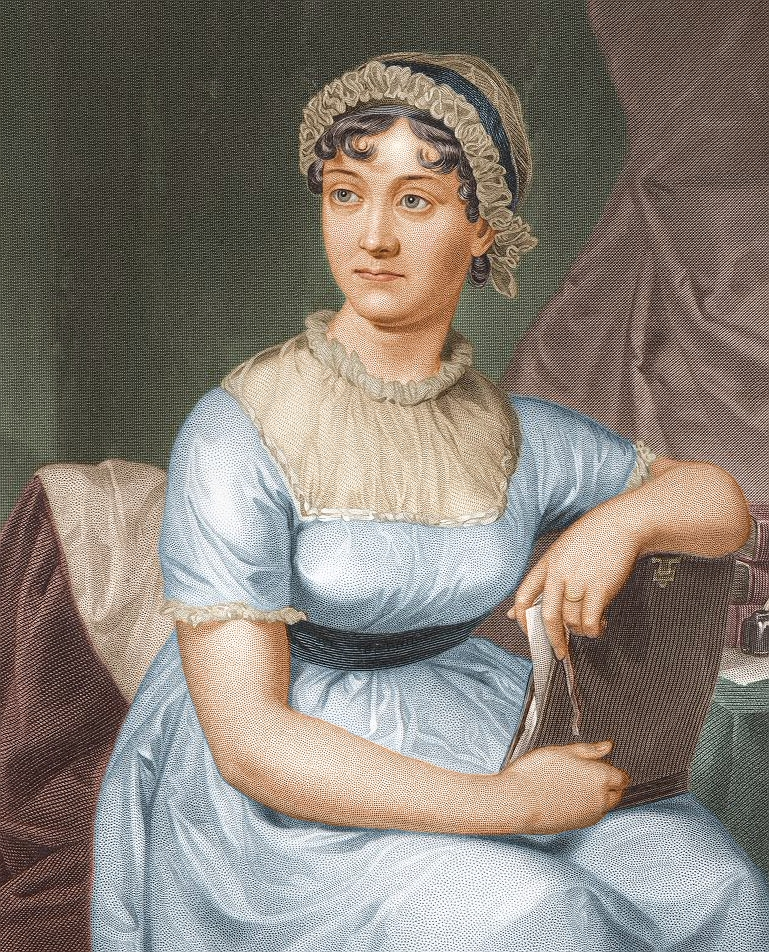
\includegraphics[scale=0.15]{chapters/img/Jane_Austen_coloured_version.jpg}
    \caption{Jane Austen}
    \label{fig:LME_Austen}
\end{wrapfigure}

It is not, however, just the frequency\is{frequency} at which we can find the progressive in the materials from Late Modern English that signals a change. What started changing about the progressive in this period was also the range of its uses. For one thing, an increasing number of specific verbs started occurring in the progressive form. Verbs describing the scene were particularly prone to being used in this form. For example, Jane Austen\ia{Austen, Jane} was linguistically progressive when she adopted the progressive form in her works in her time, as evidenced in the following example:

\begin{exe}
    \ex a water party; and by some accident she was falling overboard (\textit{Emma}, 1816: Chapter 8)
\end{exe}

As \citet[79]{Beal2004} further comments on this example, ``\citet{Strang1970} suggests that Austen used the progressive experimentally in her novels. In this example, the effect is to involve the reader in watching the action as it happens, almost as an `action replay'. {[}... I{]}n Austen's\ia{Austen, Jane} time {[}this construction{]} flouted received views on grammar and logic''.

\begin{wrapfigure}{r}{0.24\textwidth}
    \vspace{-10pt}
    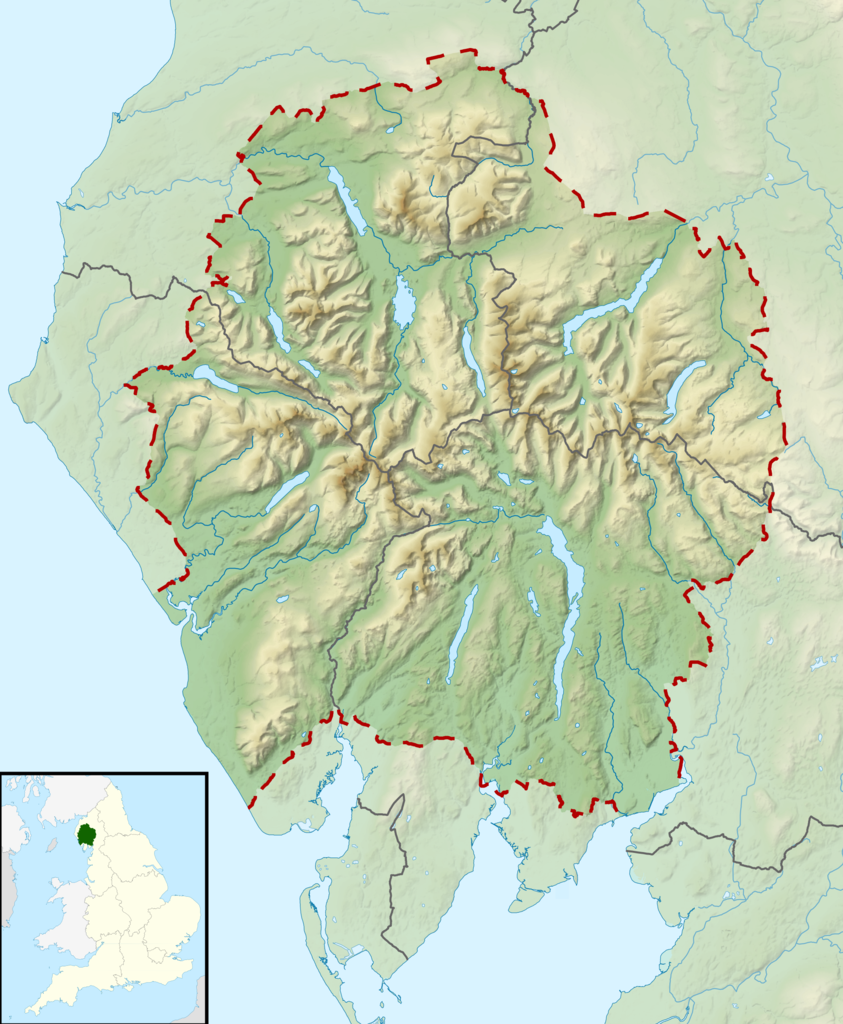
\includegraphics[scale=0.6]{chapters/img/Lake_District.png}
    \caption{Location of the Lake District, place of residence of the Lake Poets.\is{poetry} (Map by Nilfanion based on OS data, licensed under CC-BY-SA 3.0)}
    \label{fig:LakeDistrict}
\end{wrapfigure}

Progressives first start appearing in the active voice: it is only later that the progressive \glossterm{gl-passive}{passive}\is{passive} starts appearing as well. Thus, ``in 1700 constructions such as \textit{The house \textbf{is being built}} were ungrammatical but by 1900 they were normal'' \citep[66]{Beal2004}. Its rise takes place gradually between the end of the 18th century and the middle of the 20th \citep{Hundt2004passival}. The use of the progressive passive was still looked upon with a disapproving eye by some in the first half of the 20th century. It was considered not only ``clumsy'' \citep[82]{Beal2004} but also ``barbarous'', ``despicable'', and ``in bad taste'', and criticism of the progressive passive\is{passive} was particularly vitriolic in America \citep{Anderwald2014}, though today it is not considered objectionable even by the crustiest of prescriptivists.\is{prescriptivism}

Jane Austen was not the only innovative member of the literati. \citet{PraatDenison2001} show that the Southey-Coleridge cirle (the Lake\is{poetry} Poets),\footnote{The members included Dorothy\ia{Wordsworth, Dorothy} and William Wordsworth,\ia{Wordsworth, William} Robert Southey,\ia{Southey, Robert} Samuel Taylor Coleridge,\ia{Coleridge, Samuel Taylor} Charles\ia{Lamb, Charles} and Mary Lamb,\ia{Lamb, Mary} and Mary \ia{Shelley, Mary} and Percy Shelley.\ia{Shelley, Percy}} who formed a close-knit type of group, were some of the first to use the progressive passive,\is{passive} with the earliest examples dating to the second half of the 18th century. \citet[416]{PraatDenison2001} argue that

\begin{quote}
    In the politicised English literary world of the decades around 1800, with its aggressive reviews, often highly critical about diction, it is certainly possible that consciously or otherwise, groups of literary people might have wanted to distance themselves from other, older and more conservative groups.
\end{quote}
So, the progressive passive\is{passive} may have served as a marker of a group identity, this group identity being that of the Lake Poets, young individuals, and those with political views similar to those of the Lake Poets.\is{poetry} It is also not surprising then that this linguistic innovation was seen as ``monstrous'' by many, particularly those who did not belong to this group and who did not share the same worldviews.\footnote{See \citet[418--419]{PraatDenison2001} and \citet{vanBergen2013} if you want to know more.}


\begin{miscbox}{I'm lovin' it}
To the disapproval of some, in 2003 McDonald's released an advertising campaign with the slogan \textit{I'm lovin' it}.\footnote{See \url{http://www.macmillandictionaryblog.com/lovin-it}.\is{dictionaries}} Is this evidence of language change? Are we observing the same type of disapproval that the progressive passive\is{passive} received in Late Modern English? \citet{Freund2016} conducted an analysis including a range of methodological approaches and found that it is specific verbs, \textit{love} and \textit{think}, that are being used more frequently\is{frequency} in the progressive in Present Day English. \citet{Anderwald2017}, using \glossterm{gl-corpus}{corpus}\is{corpora} data from historical and Present Day American English, also proposes that the rise of the progressive with \textit{love} is due to a change in the meaning of \textit{love}, which is becoming semantically bleached to yield a meaning more like `like' or `enjoy'. Both \citet{Freund2016} and \citet{Anderwald2017} argue that it is not the whole class of \glossterm{gl-stative}{stative} verbs that has been experiencing the rise of the progressive as such. Furthermore, the now famous \textit{I'm lovin' it} phrase associated with McEnglish\footnote{See \url{https://www.urbandictionary.com/define.php?term=McEnglish}.} in fact shows patterns attested already in early 19th-century English \citep[162--163]{AartsCloseWallis2010}.\is{progressive|)}\is{aspect|)}
\end{miscbox}


\subsection{Semi-modals}\label{LME-semimodals}\is{modals|(}
Do you use verbal constructions such as those found in the following examples?

\begin{exe}
    \ex\label{ex-gonna} I'm \textbf{going to/gonna} do some bumblebee\is{bumblebees} spotting.
    \ex Do you \textbf{want to/wanna} come?
    \ex You \textbf{have to/hafta} know all about bumblebees.
    \ex\label{ex-gotta} You've \textbf{got to/gotta} love bumblebees.\is{bumblebees}
\end{exe}

\noindent Congratulations, you're a user of semi-modal constructions! As the name implies, semi-modal verbs can behave like true modals (modal auxiliaries)\is{auxiliaries} in some ways, but not in others. A fuller discussion of the auxiliaries\is{auxiliaries} can be found in the next chapter (\sectref{EModE-do}), so here we keep it brief.

The verbs \textit{be}, \textit{have}, and \textit{do} are auxiliaries,\is{auxiliaries} and here are some examples:

\begin{exe}
    \ex \textbf{Are} you looking forward to reading more about semi-modals?
    \ex \textbf{Have} you ever heard that the word \textit{corgi} originates in \ili{Welsh}? (It means `a dwarf-dog'.)
    \ex \textbf{Did} you know that the word \textit{penguin} may originate from the Welsh \textit{pen gwyn} `white head'?
\end{exe}

\noindent These three verbs are used to form various types of periphrastic tense and aspect\is{aspect} constructions, like the progressive\is{progressive} discussed above. In addition to these three auxiliaries,\is{auxiliaries} there are also modal auxiliaries,\is{auxiliaries} such as \textit{can}, \textit{will}, and \textit{must}, as in (\ref{ex-can}) below. These English modals share a number of morphological and syntactic properties, and all belong to the semantic domain of modality, which is concerned with possibility, necessity, ability, desire, and obligation. The history and current status of these ``true'' modals are discussed in \sectref{ME-modals}.

\begin{exe}
    \ex\label{ex-can} \textbf{Can} we tempt you with another example about bumblebees?\is{bumblebees}
\end{exe}

\noindent Another construction that increased in frequency\is{frequency} in the Late Modern English period is semi-modals. Semi-modals (also known as quasi-modals or emerging modals) have modal meanings, like true modals. The core semi-modals are \textit{have to} (or \textit{hafta}), (\textit{have}) \textit{got to} (or \textit{gotta}), \textit{want to} (or \textit{wanna}), and \textit{going to} (or \textit{gonna}). Another semi-modal found in some varieties is \textit{fixing to} (or \textit{finna}).\is{\emph{fixing to} (\emph{finna})}

The semi-modals share some syntactic properties with the true modals: for instance, unlike most normal lexical verbs, they occur with a following non-finite verb, as in (\ref{ex-gonna})--(\ref{ex-gotta}) above. However, they do not behave quite the same way regarding their morphosyntax as modal auxiliaries\is{auxiliaries} do. Perhaps the most important difference is that, while auxiliaries\is{auxiliaries} can be found in front of the subject\is{subjects}\is{word order} as in (\ref{ex-gonna})--(\ref{ex-can}) (e.g. \textit{\textbf{Can} we ...}), this is never possible with semi-modals, as (\ref{ex-inv-gonna})--(\ref{ex-inv-gotta}) show.

\begin{exe}
    \ex\label{ex-inv-gonna} *\textbf{Going to/Gonna} I do some bumblebee spotting?\is{bumblebees}
    \ex *\textbf{Want to/Wanna} you come?
    \ex *\textbf{Have to/Hafta} you know all about bumblebees?
    \ex\label{ex-inv-gotta} *\textbf{Got to/Gotta} you love bumblebees?\is{bumblebees}
\end{exe}

\noindent So the semi-modals have a liminal status: they don't behave totally like lexical verbs, but they don't fit in as auxiliaries\is{auxiliaries} either. \citet{Krug2000} suggests that they form a group on their own.\footnote{Other potential members of the group include \textit{need} (\textit{to}) and \textit{dare} (\textit{to}), and \textit{fixing to}. To keep things relatively simple, we'll focus on the five that are mentioned in the main text, but we'll come back to \textit{fixing to} later in this section.}

The history of \textit{going to} has been abundantly researched. Like the history of negative contraction, discussed in \sectref{LME-contraction}, it's a typical example of \glossterm{gl-grammaticalization}{grammaticalization}.\is{grammaticalization} The first instance of this construction used as a marker of intention and futurity\is{futurity} (rather than as a simple lexical verb of motion) is dated to 1482. However, it was not until the mid-17th century that its frequency\is{frequency} as a future marker started to increase, and it was not until the end of the 18th century (i.e. Late Modern English) that it became ``firmly entrenched in usage'' \citep[318--319]{PoplackTagliamonte2000}. In Present Day English, it is the second most frequent\is{frequency} future\is{futurity} marker \citep[319]{PoplackTagliamonte2000}, at least in standard Englishes. The traditional textbook account of the historical trajectory of \textit{going to} is the following:

\begin{enumerate}
    \item First we get a verb of motion used in the present progressive\is{progressive} (\textit{I'm \textbf{going to} town}).
    \item Then we start seeing a verbal construction indicating a goal/intention/determination (\textit{Some day somehow I'm \textbf{gonna} make it alright but not right now}, as in \iai{Nickelback}'s 2003 song titled \emph{Someday}).
    \item Finally, we see a verbal construction indicating a prediction, e.g. \textit{Am I really \textbf{gonna} go sixty years without cancer again?} \citep{Rees2017}.
\end{enumerate}

\noindent The contracted form, \textit{gonna}, has received some negative criticism from prescriptivists,\is{prescriptivism} especially in writing: \citet[2]{Lorenz2012} reports the claim that ``there is no word `gonna'{''}. As we know, though, what makes a word a word is whether people use it as such, and the spelling\is{orthography} \textit{gonna} is much closer to the usual pronunciation than \textit{going to} is. Like \textit{gotta}, \textit{wanna} and \textit{hafta}, the semi-modal \textit{gonna} is very well established in Present Day English.\is{futurity}

\citet{Krug2000} shows that the semi-modals -- or ``emerging modals'', as he prefers to call them -- underwent a cluster of rapid changes between 1850 and 1950, even if this is not always reflected in the word's spelling.\is{orthography} For instance, it's basically impossible to insert anything between the body of the verb and \textit{to}, e.g. *\textit{I'm \textbf{going} soon \textbf{to} be sick} or *\textit{I \textbf{want} quickly \textbf{to} come}. This shows that the \textit{to} has become \glossterm{gl-univerbation}{univerbated} with the body of the verb, and that they now form a single word in most Englishes -- similarly to what we saw with negative contraction\is{negation} in \sectref{LME-contraction} above.

As with the other phenomena we introduced in this chapter, there is regional variation\is{regional variation} in use of the semi-modals as well. In general, semi-modals are used more in American English\il{English, American} than in British English.\il{English, British} \textit{Wanna} in particular is sometimes thought to be an exclusively American English form -- but \citet[153--155]{Krug2000} shows that \textit{wanna} is used a fifth of the time in the spoken part of the British National \glossterm{gl-corpus}{Corpus}\is{corpora} (containing British English from the 1960s to the 1990s), and its frequency\is{frequency} increases every year between 1990 and 1997 in the British newspaper \textit{The Guardian}. Just like the subjunctive\is{subjunctive} discussed in \sectref{LModE-subjunctive} above, then, semi-modals are a feature of both British and American Englishes,\il{English, British}\il{English, American} even if they're more characteristic of the latter. \citet[8]{Lorenz2012} suggests that during the 19th and 20th centuries the semi-modals have been steadily replacing the core modals in both varieties.

One semi-modal with a very specific regional\is{regional variation} distribution is \textit{fixing to}.\is{\emph{fixing to} (\emph{finna})|(} This has the meaning of `{[}settling{]} one's mind or {[}deciding{]}' \citep[13]{Smith2009} and/or involves an ``immediacy {[}...{]} after a period of short delay'' and ``preparatory activity in order for the main action to be taken'' \citep[335]{Ching1987}. Here are some examples \citep[13, 17]{Smith2009}: 
\begin{exe}
    \ex I thought you knew they were \textbf{fixing to} run away and get married.
    \ex I'm \textbf{fixing to} go to a university and I am \textbf{fixing to} have some hard classes.
\end{exe}
The construction has a range of forms, including \textit{fixin' to} and \textit{finna} /fɪnə/. It originated in the south of the US in the 18th century and, although stigmatized, it has been spreading beyond the south of the country \citep{Smith2009}. As \citet[17]{Smith2009} shows, some users of \textit{fixing to} get prescriptive reactions in online forums such as ``Go to school and get an education. Your grammar sucks. How about ``fixing'' to do that!''. Although we present this interesting Southern American English\il{English, Southern American} innovation here very briefly, \citet{Ching1987} demonstrates that it is a semantically and pragmatically complex (and fascinating) phenomenon, involving nuances to do with signalling procrastination and psyching oneself up to do an action \citep[336]{Ching1987}. Importantly, \textit{fixing to} cannot simply substitute \textit{going to} or \textit{will}, and thereby stands to show that regional variation\is{regional variation} can present us with structural and pragmatic complexities not necessarily present in standard varieties of a language.\is{\emph{fixing to} (\emph{finna})|)}

\begin{figure}
    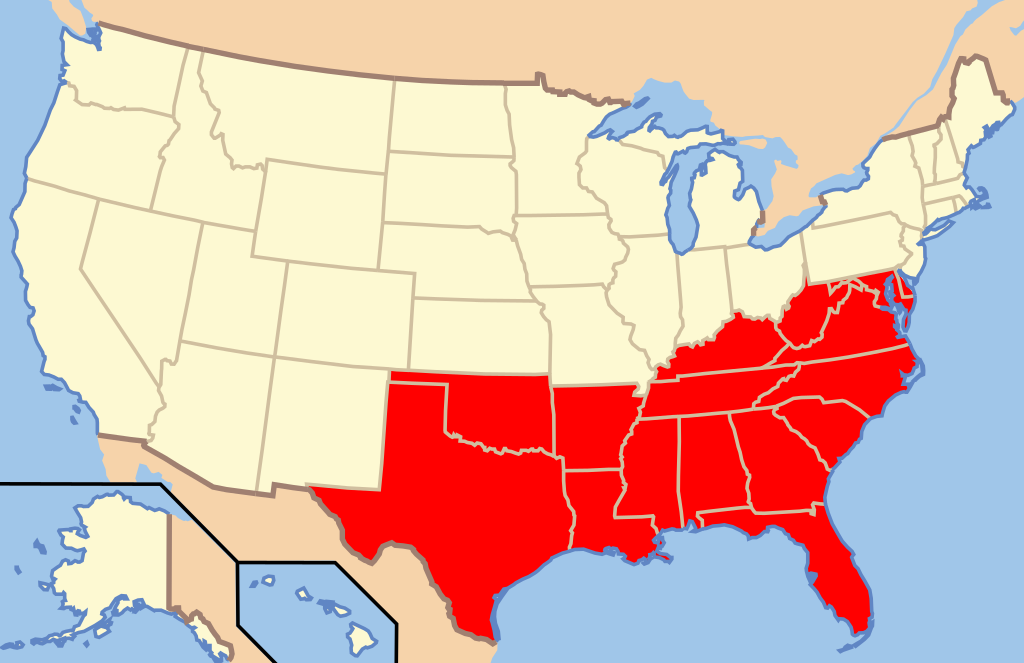
\includegraphics[width=\textwidth]{chapters/img/1024px-Map_of_USA_South.svg.png}
    \caption{American South, shown in red. (Map by Pharexia, licensed under CC-BY-SA 3.0)}
    \label{fig:American South}
\end{figure}

Overall, the semi-modals increased substantially in use during the Late Modern English period, and it seems like they are here to stay -- despite fierce opposition from prescriptivists.\is{prescriptivism} More research is still needed on the use of semi-modals outside British and American English.\il{English, British}\il{English, American}\is{modals|)}


\begin{soundbox}{/ng/ clusters through time}
\is{clusters (consonant)}
Constructions such as \textit{fixing to} are interesting from a phonological point of view as well. First of all, they show the alteration between the standard /ɪŋ/ pronunciation of the -\textit{ing} \glossterm{gl-morpheme}{morpheme} with the non-standard /ɪn/, which has been subject to plenty of sociolinguistic studies.\is{sociolinguistics} A different phenomenon, similarly frequently investigated, is that of the so-called ``velar nasal plus''. In standard Englishes, any time we find <ng> in the spelling,\is{orthography} this corresponds to the velar nasal consonant\is{consonants} /ŋ/, apart from where this is found morpheme-internally (e.g. \textit{anger} and \textit{finger}) or when the morpheme following this <ng> is the comparative or the superlative \textit{er} and \textit{est}, respectively. In these cases, what we say is /ng/ instead, i.e. one more consonant\is{consonants} -- plus one! As the spelling\is{orthography} suggests, /ng/ represents an older state of affairs. In some Present Day English dialects, <ng> in words such as \textit{sing} is still pronounced as /ng/.
\end{soundbox}


\section{Lexicon}
As mentioned earlier, Late Modern English is characterized by prescriptivism\is{prescriptivism} and by diverging developments in American and British English.\il{English, American}\il{English, British} We will therefore focus on two closely related aspects of the Late Modern English lexicon here. First, we will introduce you to two semantic processes strongly linked to social evaluation\is{evaluation problem} by language users: amelioration\is{amelioration} and pejoration.\is{pejoration} Next, we will discuss Americanisms\is{Americanisms} and their reception in Britain at the times, and we'll see yet again how common negative attitudes towards linguistic innovations are -- and how futile!

\subsection{Amelioration and pejoration}\label{LModE-pejoration}\is{amelioration|(}\is{pejoration|(}
Let's start with pejoration first, in the overall spirit of this chapter. The word \textit{spinster} used to refer to `a woman who spins' (OED, \glossterm{gl-sv}{s.v.} spinster, n.). Today, it has rather negative connotations: it's not desirable for a woman to be a spinster, `an old maid'. In contrast, the word \textit{bachelor} does not carry such negative associations. This process of obtaining negative connotations is known as \glossterm{gl-pejoration}{pejoration}, or degeneration, and involves negative value judgement. Here are some other words that have undergone this process:

\begin{itemize}
    \item \textit{amateur} (`one who loves or is fond of' > `one who cultivates anything as a pastime, as distinguished from one who prosecutes it professionally; dabbler, or superficial student or worker'; OED, \glossterm{gl-sv}{s.v.} amateur, n.)
    \item \textit{silly} (`blessed, fortunate' > `lacking in judgement or common sense'; OED, \glossterm{gl-sv}{s.v.} silly, adj., n., and adv.)
    \item \textit{mistress} (`a woman having control or authority' > `a woman other than his wife with whom a man has a long-lasting sexual relationship'; OED, \glossterm{gl-sv}{s.v.} mistress, n. and adj.)
    \item \textit{villain} (`a low-born base-minded rustic' > `an unprincipled or depraved scoundrel; a man naturally disposed to base or criminal actions, or deeply involved in the commission of disgraceful crimes'; OED, \glossterm{gl-sv}{s.v.} villain, n.).
\end{itemize}

\noindent You'll look at some more in Exercise \ref{exercise-semchange}.

On the other hand, \textsc{amelioration}, also known as elevation, involves a positive value judgement. A word that used to have negative or neutral associations gains more positive ones. Some of these words include \textit{dude}, originally `a man who shows an ostentatious regard for fashion and style in regard to dress or appearance; a dandy, a fop' and now primarily `a person (usually a man) regarded as being `cool' or fashionable, or as embodying some other admirable or desirable quality' (OED, \glossterm{gl-sv}{s.v.} dude, n., adj., and int.). Some other examples include \textit{knight} (`a boy or lad employed as an attendant or servant' > e.g. `[one] in recognition of personal merit, or as a reward for services rendered to the crown or country'; OED, \glossterm{gl-sv}{s.v.} knight, n.) and \textit{pretty} (`cunning, crafty' > `attractive and pleasing in appearance'; OED, \glossterm{gl-sv}{s.v.} pretty, adj., n., and int.), and again you'll see some more on your own in Exercise \ref{exercise-semchange}.

It may not be straightforward to decide whether a word has undergone amelioration or pejoration. Thus, \citet[205]{MillHay2018} notably remark that ``[a] possible example of amelioration during [the Middle English period] might be, depending on one's viewpoint, the word \textit{dizzy}. In [the Old English period] it meant `foolish', a meaning that survives marginally in such expressions as \textit{a dizzy blonde}; but by [Middle English] its primary meaning was `suffering from vertigo'.'' The semantic complexities are not limited just to one's point of view though, i.e. just to whether or not a semantic change is seen as positive or negative. Some words may have genuinely undergone both amelioration and pejoration in different stages in their history. And this can also be subject to region-specific\is{regional variation} differences, as in the case of \textit{homely}, which has come to mean `cosy, comfortable' in British English,\il{English, British} but which has come to mean `of plain appearance, unattractive' in North America\il{English, American} (OED, \glossterm{gl-sv}{s.v.} \emph{homely}, adj.).\footnote{We're simplifying here. But why don't you check out the entry for yourself, to discover all of the meanings of this word at different stages of the history of the language, and to find out more?}

To take a more recent example of potential pejoration, we can consider the word \textit{clever}: ``Although \textit{clever} is typically favorable today, signs of its ultimate degeneration appear in such expressions as `too clever by half' and `too clever for one's own good'{''} \citep[289]{MillHay2018}.\footnote{We took inspiration for most of these examples primarily from \citet{Campbell2013} and \citet[205 and 289]{MillHay2018}.}

We may wonder how the processes of pejoration and amelioration come about exactly, and why. These are very good questions to ask, and the answers to them are complex because we need to analyse specific words case by case, paying attention to the contexts in which these are used across decades and centuries. Let's consider one example here. \citet{Lakoff1973}, who focuses on gender\is{gender studies} asymmetries in American society of the twentieth century, points out that these asymmetries are reflected in lexical ``pairs'' such as \textit{spinster} and \textit{bachelor}, or the need to distinguish between \textit{Miss} and \textit{Mrs} for women while for men \textit{Mr} seems to suffice. One could therefore suggest that the more negative connotations of \textit{spinster} (as opposed to \textit{bachelor}) reflect societal context and developments, and this semantic change thus has to be explored through a careful analysis of the details belonging to the fields of historical sociology and gender studies here.\is{gender studies} The more negative meaning of the word, that of `[a] woman still unmarried' and `one beyond the usual age for marriage, an old maid' in particular (OED, \glossterm{gl-sv}{s.v.} spinster, n.), enters the scene during the Late Modern English period.\is{amelioration|)}\is{pejoration|)}


\begin{miscbox}{Taboos and euphemisms: you know who...}
Certain aspects of life may be considered taboo\is{taboo} in different communities and societies. Typically, these are related to excretion (to do with menstruation, peeing, pooing, and throwing up, for instance), sexual intercourse, death, and beings who are feared. When a word is considered to be too direct, another word (considered less direct, or somehow milder) is used instead -- a \textit{euphemism}. Well, at least until this euphemism becomes too directly associated with the concept and there's a need for a new euphemism yet again. Menstruation seems to be a topic giving rise to plenty of lexical variation. Some speakers may prefer to refer to the event as \textit{lady time}, \textit{Aunt Flo}, \textit{the crimson wave}, \textit{shark week}, and \textit{the monthly visitor}.\footnote{Or so at least \textit{The Independent} claims: \url{https://www.independent.co.uk/life-style/health-and-families/menstruation-study-finds-over-5000-slang-terms-for-period-a6905021.html}.} From the realm of beings that are feared or should not be mentioned, we can throw in \textit{Old Nick} (for the Devil) and \textit{He-Who-Must-Not-Be-Named} (referring to Lord Voldemort in \textit{Harry Potter}). A similar phenomenon can be observed when we avoid swearing with expressions that may be perceived as strong by some, e.g. \textit{fucking hell}, \textit{bloody hell}, \textit{holy smokes}, \textit{shit}, and \textit{for fuck's sake}, among many others. The following would most likely be perceived as rather harmless: \textit{fudge}, \textit{gosh}, \textit{shoot}, and \textit{zoonds}. \citet{Campbell2013} also gives the interesting examples of euphemisms coined in American English\il{English, American} but not in British English,\il{English, British} resulting in the following variants: \textit{ass} vs. \textit{donkey}, and \textit{cock} vs. \textit{rooster}. When it comes to the place where humans excrete, the lexical variation becomes more complex. Interestingly, one of the reviewers of this chapter noted that ``[t]he section on taboo and euphemisms is somewhat embarrassing in its length and explicitness''. As we can see, people do tend to feel strongly about taboos, and the stigma attached to these leads to the constant fuel of lexical innovation as discussed here.
\end{miscbox}


\subsection{As American as apple pie?}\il{English, American|(}\is{Americanisms|(}
Typically, when a discussion gets started about language change and dialects, the first examples that are mentioned in conversation pertain to the lexicon. One thing is called X in this region,\is{regional variation} but Y in another. Today, we might say without much hesitation that \textit{fall}, rather than \textit{autumn}, and \textit{zee} for the letter Z, rather than \textit{zed}, are typical American words -- in other words, Americanisms. The term ``Americanism'' was introduced in 1781 \citep[68]{Fisher2001}. But deciding whether or not a phrase is an Americanism is not as straightforward as may first meet the eye. For example, although some words and expressions may have been coined in North America, others might predate colonization\is{colonialism} and in fact date back to what used to be -- but no longer is -- the preferred word or expression in other varieties of English, and British English\il{English, British} in particular. In what follows, we rely on \citet{CassidyHall2001}, who distinguish so-called \glossterm{gl-synchronic}{synchronic} and \glossterm{gl-diachronic}{diachronic} Americanisms.

Synchronic Americanisms are those words and expressions that are used primarily in the US in Present Day English. Diachronic Americanisms are those words and expressions that were coined in North America, but which are not necessarily used solely in the US in the 21st century. Thus, as \citet{CassidyHall2001} aptly say, there is some tension in saying that something is ``as American as apple pie''.

Let's have a look at a couple of diachronic Americanisms. Often, when interacting with new cultures and coming across new fauna, flora, and various other aspects of life and the universe, the lexicon needs to be enriched in one way or other so that these new aspects of life can be referred to. This naturally happened also during the colonization\is{colonialism} of North America. The first wave of diachronic Americanisms can therefore be thought of as consisting precisely of words borrowed\is{borrowings} from native American languages for new concepts, as in \textit{chipmunk} (from \ili{Ojibwe}), \textit{moccasin}, and \textit{raccoon} (both from \ili{Powhatan}). This sometimes happened via a detour through other languages of European colonizers\is{colonialism} (e.g. \ili{Spanish}), as in \textit{potato} (originally from \ili{Taíno}). Another way to refer to new concepts is by making use of the already existing vocabulary, as in \textit{Indian corn}, later shortened to \textit{corn}.

These are not the only words that could be labelled Americanisms. As \citet{CassidyHall2001} also mention, sometimes British English\il{English, British} experienced innovation, while the older expression continued being used in America, and ended up being perceived as American after enough time had elapsed. This is in fact what happened to \textit{fall} (vs \textit{autumn}) and \textit{zee} (vs \textit{zed}, referring to the letter <z>). So these Americanisms are synchronic ones. These examples provide us with an interesting lesson to learn: what may seem to be a synchronic oddity may once have been the norm! This is something we will see at least a couple more times in the chapters to follow. 

Finally for our purposes, what may have started as an Americanism may no longer be perceived as such. Apart from the diachronic Americanisms mentioned above, consider the following words and expressions, and decide whether you'd perceive them as Americanisms: \textit{atomic bomb}, \textit{baseball},  \textit{boot camp}, \textit{boss}, \textit{browser}, \textit{cable car}, \textit{cahoot}, \textit{campus}, \textit{chat room}, \textit{cowboy}, \textit{cupcake}, \textit{department store}, \textit{doughnut}, \textit{email}, \textit{floppy disk}, \textit{genocide}, \textit{hacker}, \textit{hip}, \textit{hydrant}, \textit{iffy}, \textit{jazz}, \textit{jive}, \textit{know-how}, \textit{Kodak}, \textit{martini}, \textit{milk shake}, \textit{OK}, \textit{parking meter}, \textit{peanut butter}, \textit{popcorn}, \textit{populist party}, \textit{radiator}, \textit{refrigerator},\footnote{Just in case you wonder, this is where \textit{fridge} comes from.} \textit{sex appeal}, \textit{sky scraper}, \textit{soap opera}, \textit{spell check}, \textit{sundae}, \textit{telegram}, \textit{to bury the hatchet}, \textit{to commute}, \textit{to download}, \textit{to get even}, \textit{to get the hang of} (\textit{something}), \textit{to lynch}, and \textit{whodunnit}. How many of those would \textit{you} consider American?\footnote{Historically speaking, all of them are!}

On a different but not unrelated note, with the emerging consciousness towards the end of the 19th century that the English spoken in the US is a form of English different from that found in Great Britain, it is not surprising that lexical differences between English spoken in the US as opposed to Great Britain began to be commented on. These comments weren't always positive. Although coining new words for new concepts is ``inevitable [...], British observers tended to designate [these] as barbarous `Americanisms'{''} \citep[68]{Fisher2001}. This is confirmed by \citet[185]{CassidyHall2001} as well:

\begin{quote}
    Americanisms -- variances from what was considered good English usage -- had to be carefully noted and judged, certainly not adopted unaware. In short, the word Americanism at first implied a certain critical caution on the part of the observer. Later it came to be used neutrally and even, with a transatlantic shift in the point of view, favorably.
\end{quote}

\noindent Today, still, we find plenty of ``juicy'' and prescriptive data, as in ``How Americanisms are killing the English language. A book released this year claims that Americanisms will have completely absorbed the English language by 2120''.\footnote{\url{http://www.bbc.com/culture/story/20170904-how-americanisms-are-killing-the-english-language}.}\il{English, American|)}\is{Americanisms|)}

\section{Final note}
As we have seen repeatedly in this chapter, variation and change are a natural state of affairs.\is{language variation and change (field)} Furthermore, social stigma of various types can get attached to linguistic variation, just like it can be attached to any other variation. This variation is only stigmatized, however, because some part of society decides to view it as inappropriate in some way or other. There is nothing inherently wrong with linguistic variant A as opposed to linguistic variant B.


\addsec{Suggested exercises}
\begin{exercises}{Fighting accentism}\is{accentism}
\paragraph*{A.}
Imagine the press approaches you to provide a specialist's opinion on the question of which English dialect is correct. Come up with an answer.

\paragraph*{B.}
Using 5 stories from the Accentism Project launched by Carrie\ia{Carrie, Erin} and Drummond\ia{Drummond, Rob}, discuss how accentism (and prescriptivism\is{prescriptivism} more generally) may affect people's lives.\footnote{\url{https://accentism.org/}.}\\

\noindent \emph{Tips for teachers:} This exercise can be used as a written assignment. Set up the maximum/minimum word count and a deadline. We recommend 400 words to be used for both parts in total -- this makes sure the students focus on answering the question and avoid waffling\is{accentism}.

\end{exercises}

\begin{exercises}{Pet peeves}
Ask three faculty members (or, if at all possible, other individuals who teach or want to become teachers) if they have any pet peeves related to language use. Ask them also why these are important to them. What are these pet peeves? Were you surprised by any of the examples given? Why (not)? How do the peeves reported by these individuals make them feel? How does this whole exercise relate to prescriptivism?\is{prescriptivism} And finally, should English teachers and university lecturers support or fight pet peeves?\footnote{This exercise was inspired by \citet{Baragona2019}, who collects a database of linguistic bêtes noires of faculty members with her history of English students.}

\end{exercises}

\begin{exercises}{To boldly go}\label{exercise-boldly}
The Star Trek franchise has made the phrase \textit{To boldly go where no man has gone before} famous. There have nevertheless been some who have criticized the grammar of this sentence: \textit{to boldly go} is an example of a split infinitive, and one should allegedly never split one's infinitives (one should instead say \textit{to go boldly}, so that the \textit{to} and the verb are right next to each other, all snuggly). Using the internet and/or other sources, find out how old the anti-split-infinitive prescriptive rule is. Be ready to present your answer to the rest of the class, including the sources you used.

\begin{figure}[H]
    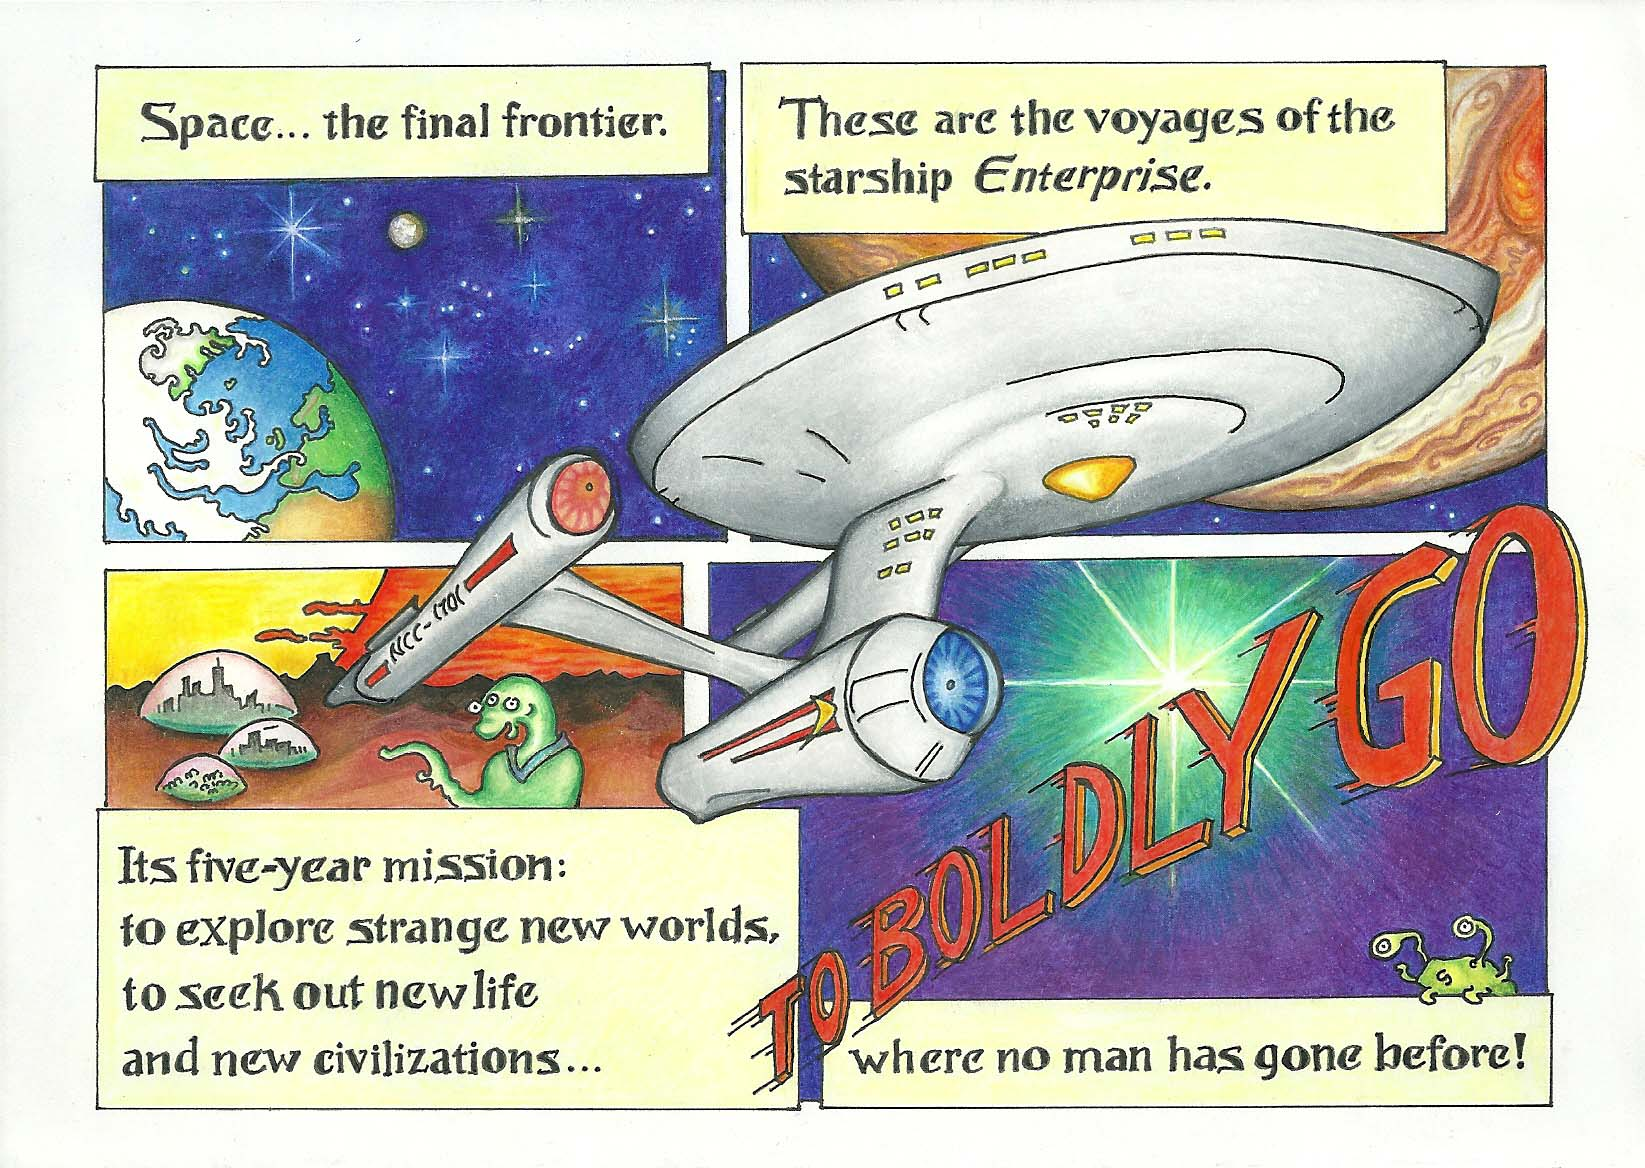
\includegraphics[width=.9\textwidth]{chapters/img/boldly.jpg}
    \caption{To boldly go; illustration kindly provided by Gry Faurholt, 2020}
    \label{fig:boldly}
\end{figure}

\noindent Earlier in the Star Trek franchise, the phrase that was used was \textit{to boldly go where no man has gone before}. It was later changed to \textit{to boldly go where no one has gone before}. Why do you think this change took place? Feel free to speculate as well as search online.

\end{exercises}

\begin{exercises}{Translating into 18th-century English}\label{exercise-backtranslate}

\sectref{LModE-morphology} and \sectref{LModE-syntax} make it clear that quite a lot has changed in the structure of English since 1700. Can you translate the text below into 1700-era English, paying particular attention to the morphological and syntactic features discussed in this chapter and chapter \ref{englishtoday}?

\begin{quote}
    I'm loving the look of the new house, but it is still being built, so I shouldn't go in there yet, even though I wanna. I would probably get hit by falling bricks and be all ``Owwww, this wasn't a good idea!'' I gotta be patient.
\end{quote}

\end{exercises}

\begin{exercises}{Tracing word formation}\label{gate}\is{word formation|(}
\emph{Note: for this exercise you will need access to the online Oxford English Dictionary\is{dictionaries} (OED) via your library or university.}\\

\noindent Look up \textit{-like} and \textit{gate} as suffixes\is{affixes} in the OED. They are labelled ``combination forms'' in the dictionary.\is{dictionaries} Answer the following questions: 
\begin{itemize}
\item When were these two suffixes first attested in the history of English? Are you surprised? Why (not)?
\item Go to ``entry profile'' (type ``ctrl+f'' and then ``entry profile'', or ``cmd+f''). In which years, approximately, were the suffixes most frequent?\is{frequency} You will find the relevant information under ``Timeline of quotation evidence''.
\item Now look at the entries that contain the suffixes (``Entries which link here''). Find 1--3 more examples with the suffixes.\is{affixes}\is{word formation|)}
\end{itemize}

\end{exercises}

\begin{exercises}{Late Modern English: seemingly the same as Present Day English?}
\chili{}

Have a look at the excerpts provided in \sectref{LModE-texts}. Can you notice any differences between these excerpts in contrast to Present Day English? Note down any differences and classify them by distinguishing the following linguistic levels:
\begin{itemize}
\item phonetics/phonology
\item orthography (i.e. spelling)\is{orthography}
\item morphology
\item syntax
\item lexicon and semantics
\item pragmatics
\end{itemize}

\noindent How many differences have you spotted? Are you surprised in any way? Why or why not? Would you say there are a lot of differences? How could one establish what amounts to ``a lot of'' differences in this context?

On a different note, can you spot any examples in the excerpts that point to prescriptivism,\is{prescriptivism} proscriptivism, or linguistic discrimination in any way?

\end{exercises}

\begin{exercises}{Gritty details and abstractions}
Look at Figure \ref{fig:NegCont} and the claim that contraction is preferred when the stem of the verb ends in a vowel,\is{vowels} a nasal, or a liquid. Does the data back this claim up?

\end{exercises}

\begin{exercises}{Looking at Americanisms}\label{exercise-Amer}\is{Americanisms|(}
\emph{Note: for this exercise you will need access to the online Oxford English Dictionary\is{dictionaries} (OED) via your library or university.}\\

\noindent Use the OED and work with the following words: \textit{to antagonize}, \textit{to belittle}, \textit{butte},  \textit{coca-cola}, \textit{cookie}, \textit{cougar}, \textit{creek} (referring to a stream-like object), \textit{funky}, \textit{lengthy}, and \textit{woodchuck}. Make sure you exploit the information available in the dictionary\is{dictionaries} to its full extent -- don't just look at the first couple of lines. Your tasks are the following:

\begin{figure}[H]
    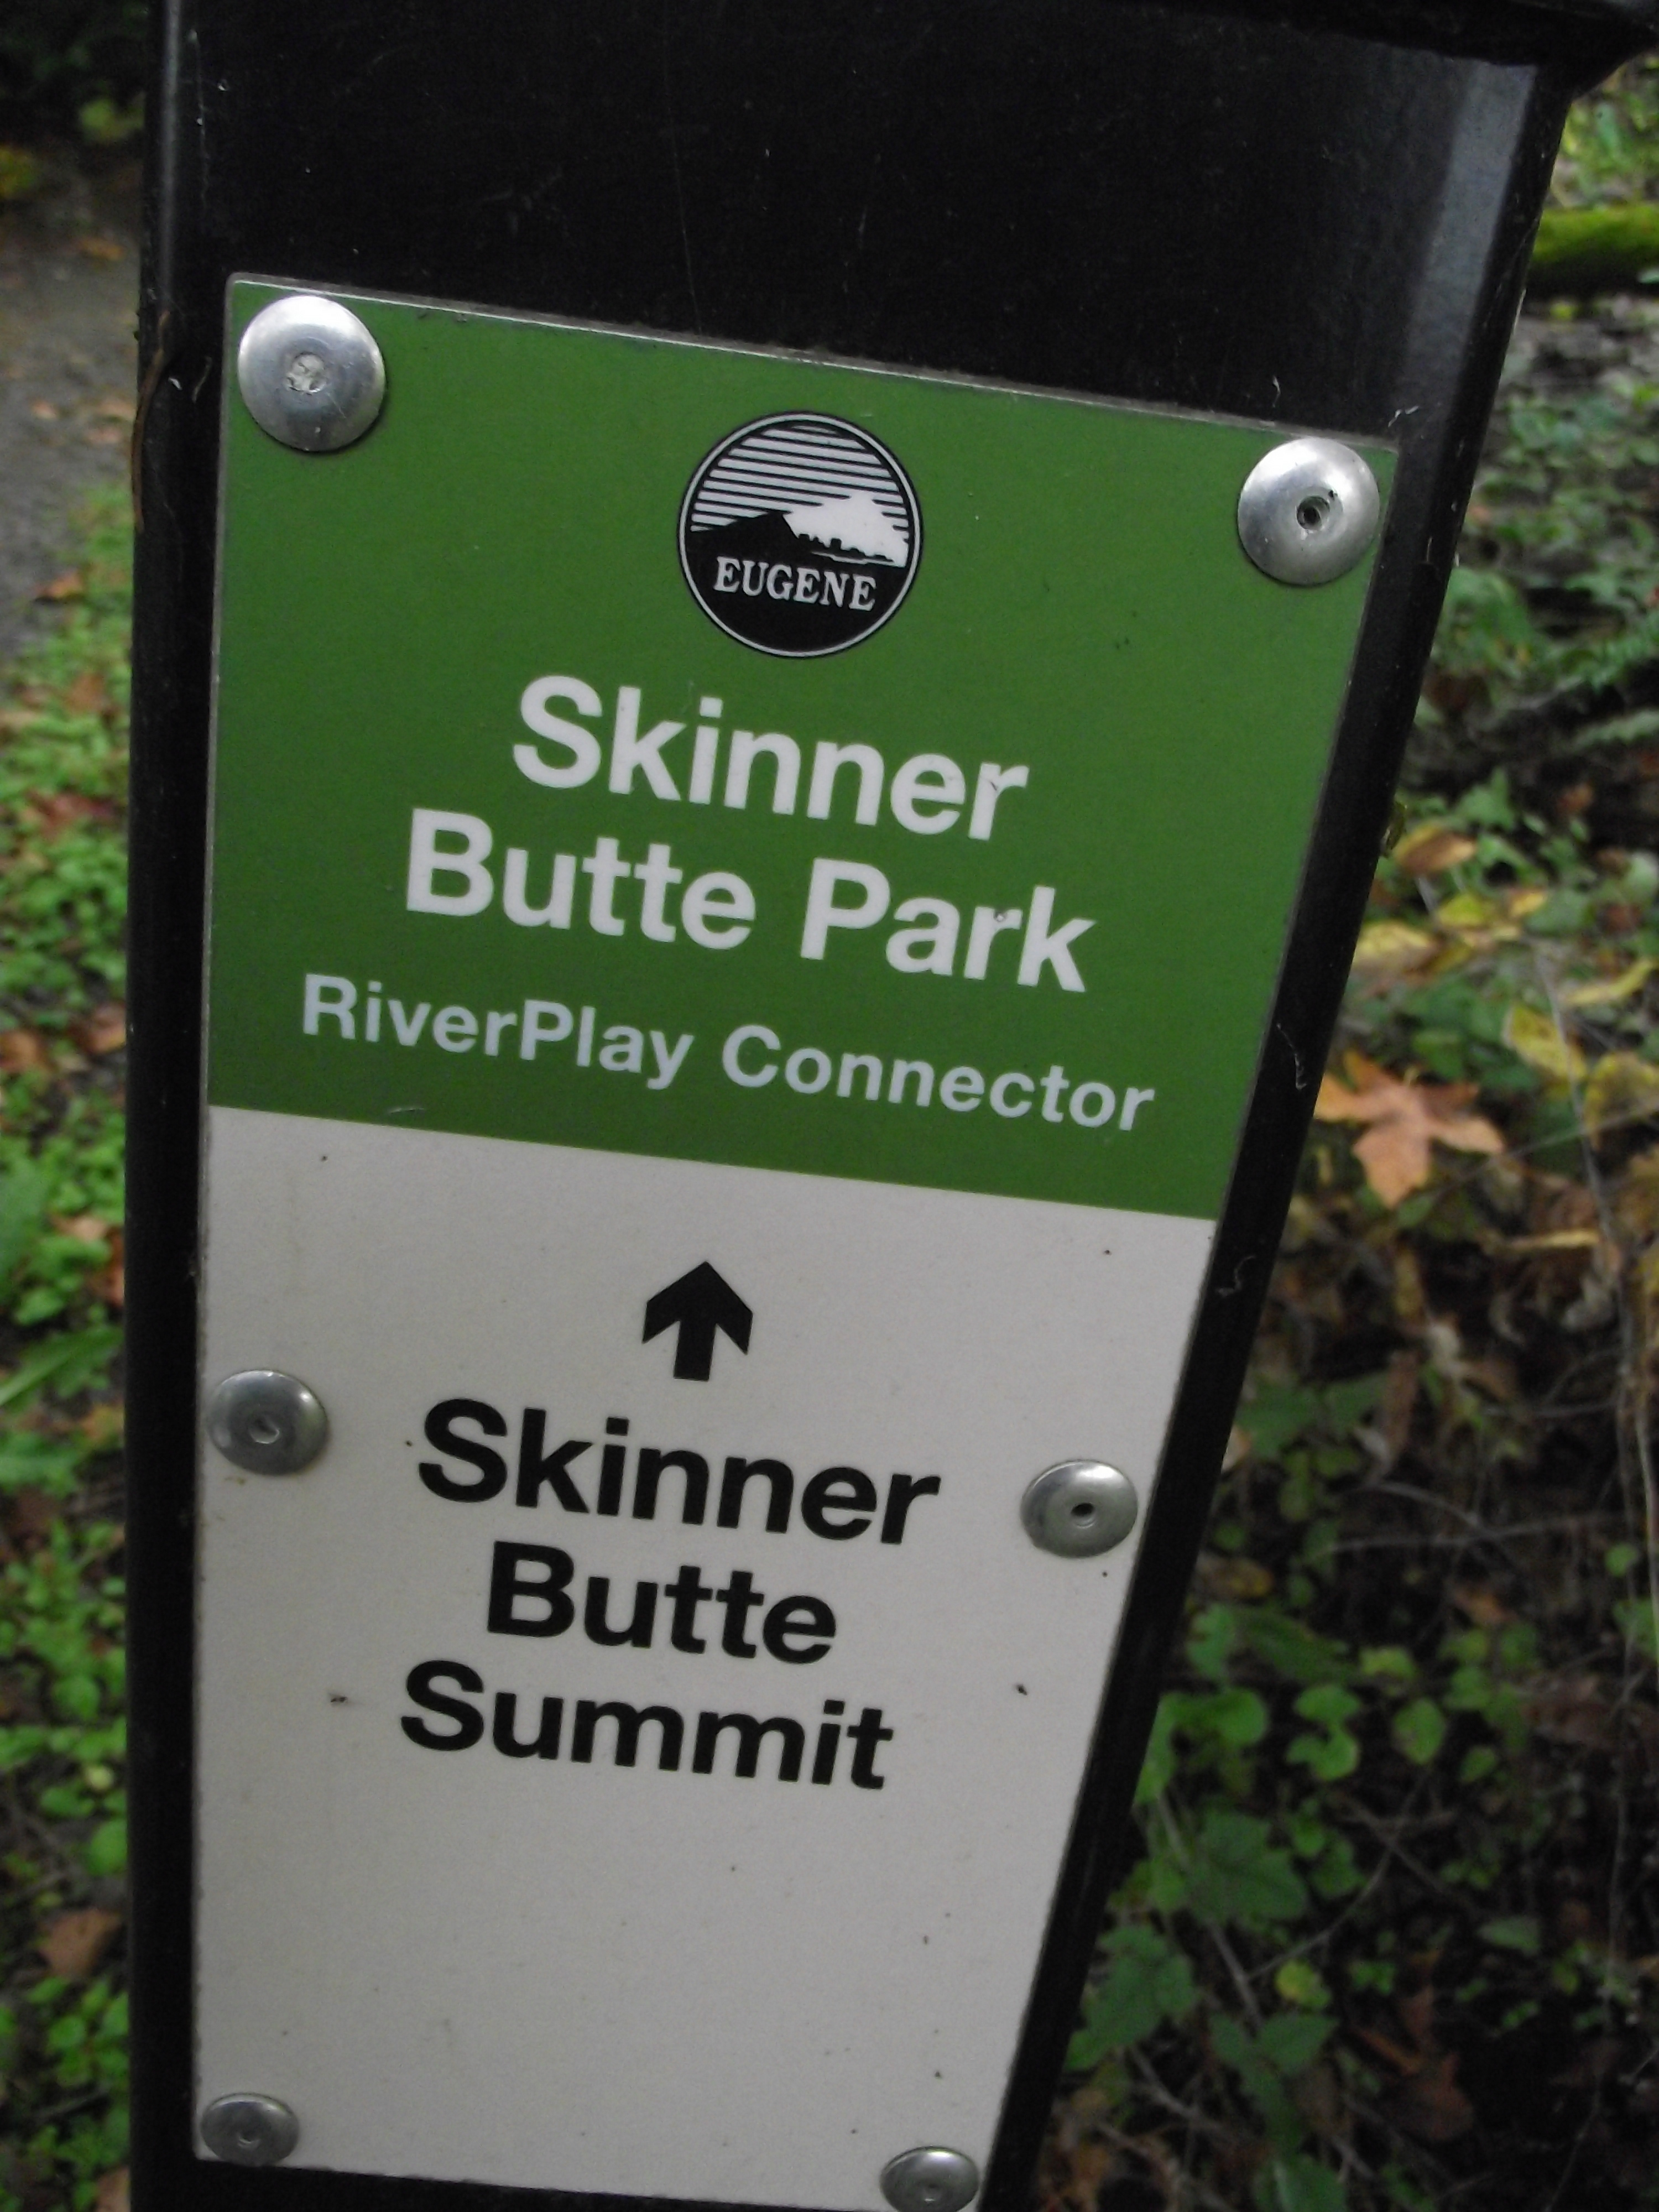
\includegraphics[width=.3\textwidth]{chapters/img/Skinner_Butte.JPG}
    \caption{On the way to Skinner Butte in Eugene, Oregon, US; photo taken by Míša in 2019}
    \label{fig:SkinnerButte}
\end{figure}


\begin{itemize}
\item If you aren't familiar with the words, do some web searching first of all to make sure you get a general sense of what these words might refer to.
\item Which of these words are restricted to North America?
\item Which of these words are restricted to specific regions\is{regional variation} in North America?
\item When is the word first attested and what is its origin (etymology)? Are you surprised in any way? Why (not)?
\item What does this say about the contact of American English\il{English, American} speakers and other cultures?
\item What makes an Americanism? What criteria should a word or an expression meet for it to count as an Americanism, in your opinion?
\end{itemize}


\noindent \emph{Tips for teachers:} Assign different words to different students/groups, or assign only a couple of the words.\is{Americanisms|)}
\end{exercises}

% \begin{figure}[H]
%     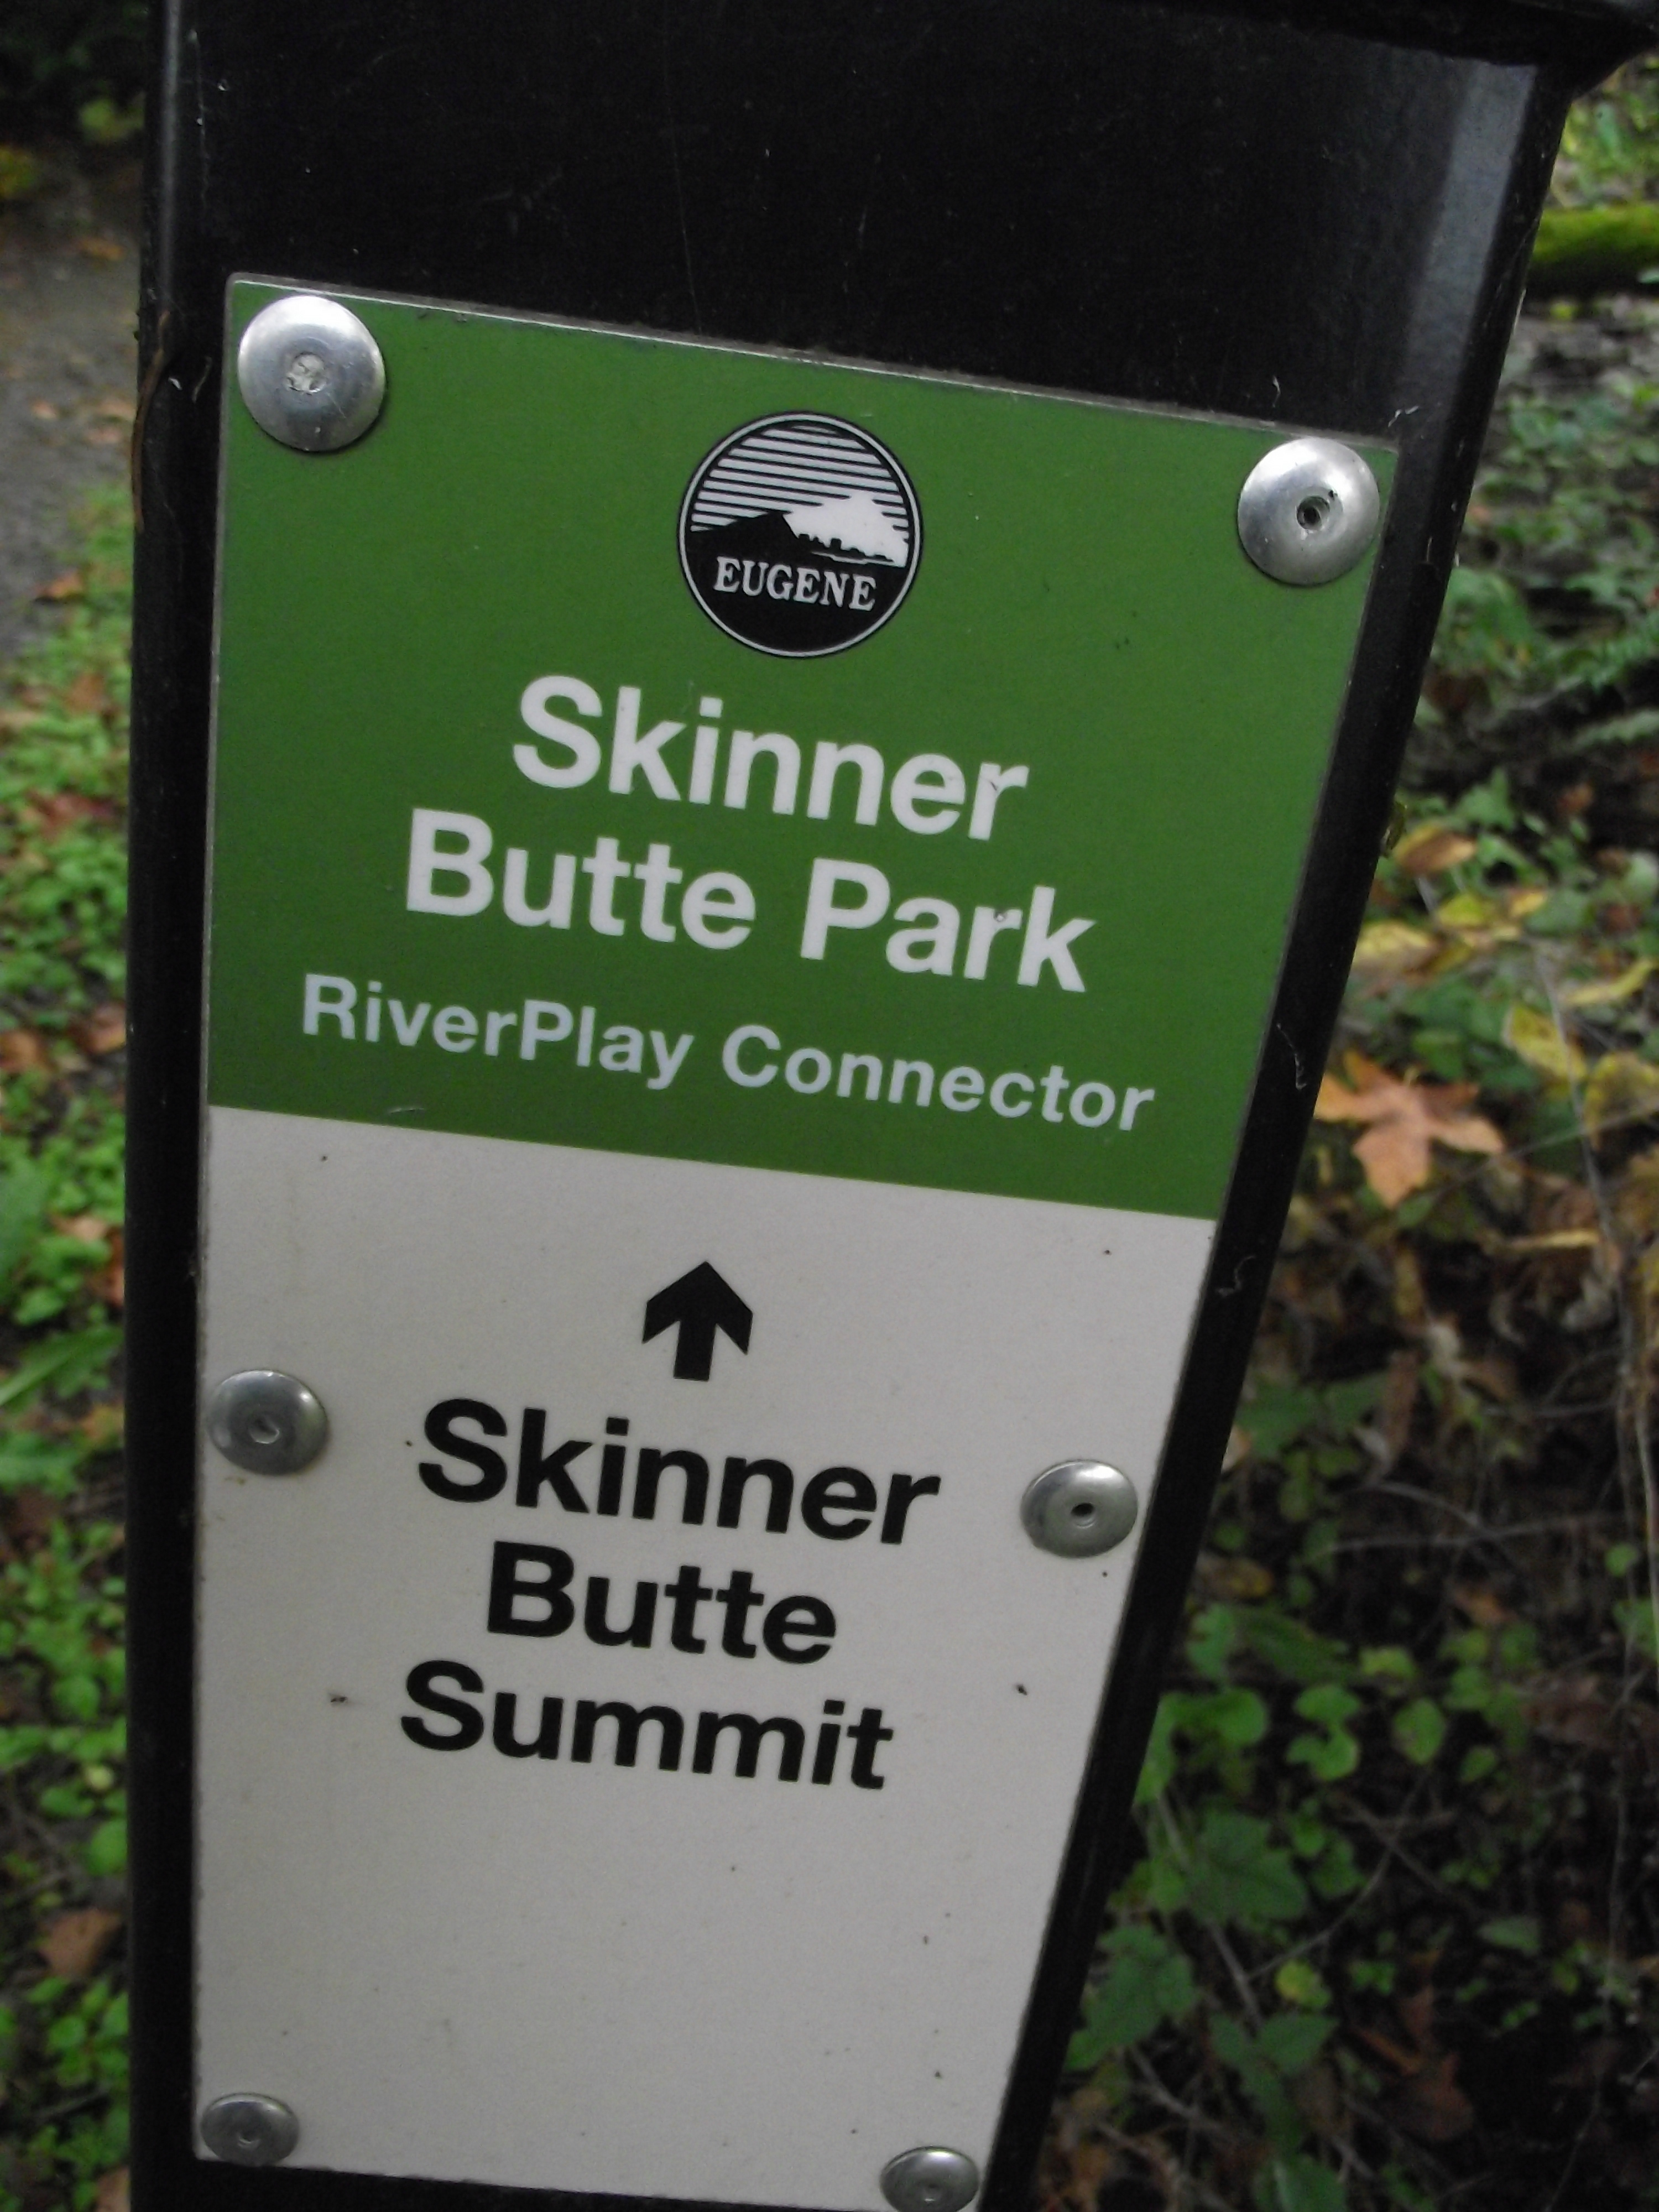
\includegraphics[width=.4\textwidth]{chapters/img/Skinner_Butte.JPG}
%     \caption{On the way to Skinner Butte in Eugene, Oregon, US; photo taken by Míša in 2019}
%     \label{fig:SkinnerButte}
% \end{figure}

\begin{exercises}{Tracing semantic change}\label{exercise-semchange}
\emph{Note: for this exercise you will need access to the online Oxford English Dictionary\is{dictionaries} (OED) via your library or university.}\\

\noindent Find the following words as nouns in the OED: \textit{baboon}, \textit{churl}, \textit{gay}, \textit{girl}, \textit{hussy}, \textit{mouse}, and \textit{weed}. Check out the following adjectives as well: \textit{artful}, \textit{coy}, \textit{crafty}, \textit{cunning}, \textit{fond}, \textit{funky}, \textit{jolly}, \textit{lewd}, \textit{nice}, \textit{shrewd}, \textit{silly}, and \textit{subtle}. Focus on these words as nouns (if they can be nouns) or as adjectives (if they aren't used as nouns). Also look at the following as verbs: \textit{to await}, \textit{to shit}, \textit{to smite}, and \textit{to tease}. Answer the following questions:


\begin{itemize}
\item Can you trace any semantic change in the history of these words?
\item If so, are there any instances of amelioration\is{amelioration} and/or pejoration?\is{pejoration}
\end{itemize}
Make sure you go through all of the meanings the dictionary entries provide. It may be a bit unusual to work with the dictionary\is{dictionaries} at first, but one of the points of this exercise is to make you get to grips with how to find information in the entries related to semantics.\\

\noindent \emph{Tips for teachers:} Assign different words to different students/groups, or assign only a couple of the words.
\end{exercises}

\begin{exercises}{Everybody poops and everybody pees}
\begin{wrapfigure}{r}{0.5\textwidth}
    \vspace*{-5mm}
    
\includegraphics[width=\textwidth]{chapters/img/toilet.jpg}
    \caption{An excretion facility in Melbourne, Victoria, Australia; photo taken by Míša in 2019}
    \label{fig:extrementation facility}
\end{wrapfigure}

Ask at least one (native or non-native) speaker of English about the words they use to refer to the object shown in Figure \ref{fig:extrementation facility}. Ask them if they know any other words for this object. Next, ask them if there's a reason why they use the one that they say they use.\footnote{Check out Tarō Gomi's\ia{Gomi, Taro} book titled \textit{Everyone Poops}.}
\vspace*{4.5cm}~
\end{exercises}

\begin{exercises}{Food for thought}
Answer the following questions. These are taken, and very slightly adapted, from \citet[52]{Hickey2019} and \citet[289]{Paraskevas2019}:\is{standardization}

\begin{enumerate}
\item In what ways do you think the notion of standard English can be beneficial? Are there any disadvantages to concentrating on standard English(es) in education?
\item What are the pros and cons of integrating non-standard language into school programmes, such as English-language arts classes? Would this change lead to more advantages for students, or would it disadvantage them?
\newpage
\item If you were to teach your own class on the history of English, would you focus on the history of standard English(es)? Why (not)?
\end{enumerate}

\noindent \emph{Tips for teachers:} This can be used as a writing exercise.\is{standardization}

\end{exercises}

\begin{exercises}{How do celebrities pronounce their /r/s?}\label{exercise-r}
Search on the web for a famous person from New York\il{English, New York} or Boston\il{English, Boston} and look up an audio(visual) interview with this person online.\footnote{Alternatively, you can simply use this video with Woody Allen\ia{Allen, Woody} (from New York): \url{https://www.youtube.com/watch?v=hpniYxRjX3o}.}

Note down all words, and all instances of words, which can be realized with a post-vocalic /r/ (e.g. \textit{car}, \textit{card}). Listen to the interview as often as necessary to answer the following:
\begin{itemize}
    \item Does your famous person always pronounce these with an /r/? If not, determine how many words do have an /r/ out of how many, e.g. 7 out of 11 words contain a post-vocalic /r/. Then calculate the percentage. Hint: if 11 is 100\%, then 0.11 is 1\%. 7 divided by 0.11 gives us 64\%.
    \item Are there any cases where you couldn’t quite decide if the /r/ was there?
\end{itemize}
	
\end{exercises}

\begin{exercises}{Morphosyntactic variation in World Englishes}
\largerpage
Using the Electronic World Atlas of Varieties of English,\footnote{\url{https://ewave-atlas.org/}.} look at the following under the ``Features'' tab, and be prepared to summarize how widespread these variants are, and in what types of English they occur:
\begin{itemize}
    \item ``7. Me instead of I in coordinate subjects''\is{subjects}
    \item ``10. No gender\is{gender (grammatical)} distinction in third person singular''
    \item ``91. DO as habitual marker''
    \item ``94. Progressive\is{progressive} marker stap or stay''
    \item ``98. After perfect''\is{aspect}
    \item a feature of your own choice that particularly intrigues you
\end{itemize}

\noindent \emph{Acknowledgement}: We would like to thank Melanie Röthlisberger\ia{Röthlisberger, Melanie} for drawing our attention to this database and suggesting that we might add an exercise based on this wonderful resource.
\end{exercises}


\addsec{Texts}
\largerpage
Late Modern English is full of texts one could look at linguistically. Below we give you just a very small taster.

\begin{texts}{Lawing and Jawing}
\label{LModE-texts}
The following is an extract from \emph{Lawing and Jawing} (originally published in 1931) in \textit{Three Plays} (2005) by Zora Neale Hurston,\ia{Hurston, Zora Neale} one of the most prominent African American\il{English, African American} authors.

\begin{quote}
    \internallinenumbers*{}
    JUDGE\phantom{XX} Hear! Hear! Court is set! My honor is on de bench.\\
    \phantom{JUDGEXX} You moufy folks set up!\\
    \phantom{JUDGEXX} (He glares at the boy with the pretty girl)\\
    \phantom{JUDGEXX} All right, Mr. Whistle-britches, just keep up dat jawing\\
    \phantom{JUDGEXX} now and see how much time I'll give you!

    BOY\phantom{XXXX} I wasn't talking, your honor.
    
    JUDGE\phantom{XX} Well, quit looking so moufy.\\
    \phantom{JUDGEXX} (to CLERK) Call de first case.\\
    \phantom{JUDGEXX} And I warn each and all dat my honor is in\\
    \phantom{JUDGEXX} bad humor dis mawnin'. I'd give a\\
    \phantom{JUDGEXX} canary bird\is{birds} twenty years for peckin' at a elephant.\\
    \phantom{JUDGEXX} (to CLERK) Bring 'em on.

    CLERK\phantom{XX} (Reading) Cliff Mullins, charged with assault upon his\\
    \phantom{CLERKXX} wife with a weapon and disturbing the peace.\\
    \phantom{CLERKXX} (As CLIFF is led to the bar by the officer, the JUDGE glares\\
    \phantom{CLERKXX} ferociously at the prisoner. His wife, all bandages, limps\\
    \phantom{CLERKXX} up to the bar at the same time.)

    JUDGE\phantom{XX} So youse one of dese hard-boiled wife-beaters, huh? Just\\
    \phantom{JUDGEXX} a mean old woman-Jessie! If I don't lay a hearing on you,\\
    \phantom{JUDGEXX} God's a gopher! Now what \emph{made} you cut such a caper?
%     \end{linenumbers}
\end{quote}
\end{texts}


\largerpage[1.5]

\begin{texts}{North and South}
\textit{North and South} is a novel written by Elizabeth C. Gaskell\ia{Gaskell, Elizabeth C.} in 1854. It presents us with characters with southern and northern English\il{English, Northern England} affiliations, who enter into relationships of various sorts.\footnote{The text is taken from the following Project Gutenberg webpage: \url{http://www.gutenberg.org/files/4276/4276-h/4276-h.htm}.}

\begin{quote}
    \internallinenumbers*{}
    ``As you please. As Dixon pleases. But, Margaret, don't get to use these horrid Milton words. ‘Slack of work:' it is a provincialism. What will your aunt Shaw say, if she hears you use it on her return?''
    
    ``Oh, mamma! don't try and make a bugbear of aunt Shaw,'' said Margaret, laughing. ``Edith picked up all sorts of military slang from Captain Lennox, and aunt Shaw never took any notice of it.''
    
    ``But yours is factory slang.''
    
    ``And if I live in a factory town, I must speak factory language when I want it. Why, mamma, I could astonish you with a great many words you never heard in your life. I don't believe you know what a knobstick is.''
    
    ``Not I, child. I only know it has a very vulgar sound; and I don't want to hear you using it.''
    
    ``Very well, dearest mother, I won't. Only I shall have to use a whole explanatory sentence instead.''
    
    ``I don't like this Milton,'' said Mrs. Hale. ``Edith is right enough in saying it's the smoke that has made me so ill.''
    
    Margaret started up as her mother said this. Her father had just entered the room, and she was most anxious that the faint impression she had seen on his mind that the Milton air had injured her mother's health, should not be deepened—should not receive any confirmation. She could not tell whether he had heard what Mrs. Hale had said or not; but she began speaking hurriedly of other things, unaware that Mr. Thornton was following him.
    
    ``Mamma is accusing me of having picked up a great deal of vulgarity since we came to Milton.''
    
    The ``vulgarity'' Margaret spoke of, referred purely to the use of local words, and the expression arose out of the conversation they had just been holding. But Mr. Thornton's brow darkened; and Margaret suddenly felt how her speech might be misunderstood by him; so, in the natural sweet desire to avoid giving unnecessary pain, she forced herself to go forwards with a little greeting, and continue what she was saying, addressing herself to him expressly.
    
    ``Now, Mr. Thornton, though ``knobstick'' has not a very pretty sound, is it not expressive? Could I do without it, in speaking of the thing it represents? If using local words is vulgar, I was very vulgar in the Forest,—was I not, mamma?''
    
    It was unusual with Margaret to obtrude her own subject of conversation on others; but, in this case, she was so anxious to prevent Mr. Thornton from feeling annoyance at the words he had accidentally overheard, that it was not until she had done speaking that she coloured all over with consciousness, more especially as Mr. Thornton seemed hardly to understand the exact gist or bearing of what she was saying, but passed her by, with a cold reserve of ceremonious movement, to speak to Mrs. Hale.
%     \end{linenumbers}
    
    ...
    
%     \begin{linenumbers}
    ``Thornton's?'' asked he. ``Ay, I've been at Thornton's''
    
    ``And what did he say?''
    
    ``Such a chap as me is not like to see the measter. Th' o'erlooker bid me go and be d——d.''
    
    ``I wish you had seen Mr. Thornton,'' said Mr. Hale. ``He might not have given you work, but he would not have used such language.''
    
    ``As to th' language, I'm welly used to it; it dunnot matter to me. I'm not nesh mysel' when I'm put out. It were th' fact that I were na wanted theer, no more nor ony other place, as I minded.''
    
    ``But I wish you had seen Mr. Thornton,'' repeated Margaret. ``Would you go again—it's a good deal to ask, I know—but would you go to-morrow and try him? I should be so glad if you would.''
    
    ``I'm afraid it would be of no use,'' said Mr. Hale, in a low voice. ``It would be better to let me speak to him.'' Margaret still looked at Higgins for his answer. Those grave soft eyes of hers were difficult to resist. He gave a great sigh.
    
    ``It would tax my pride above a bit; if it were for mysel', I could stand a deal o' clemming first; I'd sooner knock him down than ask a favour from him. I'd a deal sooner be flogged mysel'; but yo're not a common wench, axing yo'r pardon, nor yet have yo' common ways about yo'. I'll e'en make a wry face, and go at it to-morrow. Dunna yo' think that he'll do it. That man has it in him to be burnt at the stake afore he'll give in. I'll do it for yo'r sake, Miss Hale, and it's first time in my life as e'er I give way to a woman. Neither my wife nor Bess could e'er say that much again me.''
    
    ``All the more do I thank you,'' said Margaret, smiling. ``Though I don't believe you: I believe you have just given way to wife and daughter as much as most men.''
    
    ``And as to Mr. Thornton,'' said Mr. Hale, ``I'll give you a note to him, which, I think I may venture say, will ensure you a hearing.''
    
    ``I thank yo' kindly, sir, but I'd as lief stand on my own bottom. I dunnot stomach the notion of having favour curried for me, by one as doesn't know the ins and outs of the quarrel. Meddling `twixt master and man is liker meddling `twixt husband and wife than aught else: it takes a deal of wisdom to do ony good. I'll stand guard at the lodge door. I'll stand there fro' six in the morning till I get speech on him. But I'd liefer sweep th' streets, if paupers had na' got hold on that work. Dunna yo' hope, miss. There'll be more chance o' getting milk out of a flint. I wish yo' a very good night, and many thanks to yo'.''
    
    ``You'll find your shoes by the kitchen fire; I took them there to dry,'' said Margaret.
    
    He turned round and looked at her steadily, and then he brushed his lean hand across his eyes and went his way.
    
    ``How proud that man is!'' said her father, who was a little annoyed at the manner in which Higgins had declined his intercession with Mr. Thornton.
    
    ``He is,'' said Margaret; ``but what grand makings of a man there are in him, pride and all.''
%     \end{linenumbers}
\end{quote}


\end{texts}

\begin{texts}{Walden}
Here we're giving you a sample of some non-fiction as well. Henry David Thoreau's\ia{Thoreau, Henry David} \textit{Walden}, first published in 1854, presents us with American English\il{English, American} of the 19th century. Thoreau tells the readers about his life in a cabin in the woods which he built on Ralph Waldo Emerson's\ia{Emerson, Ralph Waldo} property (with the encouragement and the permission of the latter, of course).\footnote{The text is taken from the following Project Gutenberg webpage: \url{https://www.gutenberg.org/files/205/205-h/205-h.htm}.}

\begin{quote}
\internallinenumbers*{}
    I think that in the railroad car we are inclined to spend more on luxury than on safety and convenience, and it threatens without attaining these to become no better than a modern drawing room, with its divans, and ottomans, and sun-shades, and a hundred other oriental things, which we are taking west with us, invented for the ladies of the harem and the effeminate natives of the Celestial Empire, which Jonathan should be ashamed to know the names of. I would rather sit on a pumpkin and have it all to myself than be crowded on a velvet cushion. I would rather ride on earth in an ox cart with a free circulation, than go to heaven in the fancy car of an excursion train and breathe a malaria all the way.
%     \end{linenumbers}
    
    ...
    
%     \begin{linenumbers}
    I dug my cellar in the side of a hill sloping to the south, where a woodchuck had formerly dug his burrow, down through sumach and blackberry roots, and the lowest stain of vegetation, six feet square by seven deep, to a fine sand where potatoes would not freeze in any winter. The sides were left shelving, and not stoned; but the sun having never shone on them, the sand still keeps its place. It was but two hours' work. I took particular pleasure in this breaking of ground, for in almost all latitudes men dig into the earth for an equable temperature. Under the most splendid house in the city is still to be found the cellar where they store their roots as of old, and long after the superstructure has disappeared posterity remark its dent in the earth. The house is still but a sort of porch at the entrance of a burrow.
%     \end{linenumbers}
    
    ...
    
%     \begin{linenumbers}
    The next year I sometimes caught a mess of fish for my dinner, and once I went so far as to slaughter a woodchuck which ravaged my bean-field,—effect his transmigration, as a Tartar would say,—and devour him, partly for experiment's sake; but though it afforded me a momentary enjoyment, notwithstanding a musky flavor, I saw that the longest use would not make that a good practice, however it might seem to have your woodchucks ready dressed by the village butcher.
%     \end{linenumbers}
    
    ...
    
%     \begin{linenumbers}
    There is an incessant influx of novelty into the world, and yet we tolerate incredible dulness. I need only suggest what kind of sermons are still listened to in the most enlightened countries. There are such words as joy and sorrow, but they are only the burden of a psalm, sung with a nasal twang, while we believe in the ordinary and mean. We think that we can change our clothes only. It is said that the British Empire\is{British Empire} is very large and respectable, and that the United States are a first-rate power. We do not believe that a tide rises and falls behind every man which can float the British Empire like a chip, if he should ever harbor it in his mind. Who knows what sort of seventeen-year locust will next come out of the ground? The government of the world I live in was not framed, like that of Britain, in after-dinner conversations over the wine.
%     \end{linenumbers}
    
    ...
    
%     \begin{linenumbers}
    However, if one designs to construct a dwelling house, it behooves him to exercise a little Yankee shrewdness, lest after all he find himself in a workhouse, a labyrinth without a clue, a museum, an almshouse, a prison, or a splendid mausoleum instead.
%     \end{linenumbers}
    
    ...
    
%     \begin{linenumbers}
    Many a forenoon have I stolen away, preferring to spend thus the most valued part of the day; for I was rich, if not in money, in sunny hours and summer days, and spent them lavishly; nor do I regret that I did not waste more of them in the workshop or the teacher's desk. But since I left those shores the woodchoppers have still further laid them waste, and now for many a year there will be no more rambling through the aisles of the wood, with occasional vistas through which you see the water. My Muse may be excused if she is silent henceforth. How can you expect the birds\is{birds} to sing when their groves are cut down?
%     \end{linenumbers}
\end{quote}


\end{texts}

\begin{texts}{David Copperfield}
Here we give you a text sample from Charles Dickens.\ia{Dickens, Charles} \textit{David Copperfield} is a novel that was first serialized and then published in 1850 as a book. The following conversation is between two male speakers.\footnote{The text is taken from the following Project Gutenberg webpage: \url{http://www.gutenberg.org/files/766/766-h/766-h.htm\#link2HCH0039}.}

\begin{quote}
    \internallinenumbers*{}
    I had not walked out far enough to be quite clear of the town, upon the Ramsgate road, where there was a good path, when I was hailed, through the dust, by somebody behind me. The shambling figure, and the scanty great-coat, were not to be mistaken. I stopped, and Uriah Heep came up.
    
    ``Well?'' said I.
    
    ``How fast you walk!'' said he. ``My legs are pretty long, but you've given ‘em quite a job.''
    
    ``Where are you going?'' said I.
    
    ``I am going with you, Master Copperfield, if you'll allow me the pleasure of a walk with an old acquaintance.'' Saying this, with a jerk of his body, which might have been either propitiatory or derisive, he fell into step beside me.
    
    ``Uriah!'' said I, as civilly as I could, after a silence.
    
    ``Master Copperfield!'' said Uriah.
    
    ``To tell you the truth (at which you will not be offended), I came out to walk alone, because I have had so much company.''
    
    He looked at me sideways, and said with his hardest grin, ``You mean mother.''
    
    ``Why yes, I do,'' said I.
    
    ``Ah! But you know we're so very umble,'' he returned. ``And having such a knowledge of our own umbleness, we must really take care that we're not pushed to the wall by them as isn't umble. All stratagems are fair in love, sir.''
    
    Raising his great hands until they touched his chin, he rubbed them softly, and softly chuckled; looking as like a malevolent baboon, I thought, as anything human could look.
    
    ``You see,'' he said, still hugging himself in that unpleasant way, and shaking his head at me, ``you're quite a dangerous rival, Master Copperfield. You always was, you know.''
    
    ``Do you set a watch upon Miss Wickfield, and make her home no home, because of me?'' said I.
    
    ``Oh! Master Copperfield! Those are very arsh words,'' he replied.
    
    ``Put my meaning into any words you like,'' said I. ``You know what it is, Uriah, as well as I do.''
    
    ``Oh no! You must put it into words,'' he said. ``Oh, really! I couldn't myself.''
    
    ``Do you suppose,'' said I, constraining myself to be very temperate and quiet with him, on account of Agnes, ``that I regard Miss Wickfield otherwise than as a very dear sister?''
    
    ``Well, Master Copperfield,'' he replied, ``you perceive I am not bound to answer that question. You may not, you know. But then, you see, you may!''
    
    Anything to equal the low cunning of his visage, and of his shadowless eyes without the ghost of an eyelash, I never saw.
    
    ``Come then!'' said I. ``For the sake of Miss Wickfield—''
    
    ``My Agnes!'' he exclaimed, with a sickly, angular contortion of himself. ``Would you be so good as call her Agnes, Master Copperfield!''
    
    ``For the sake of Agnes Wickfield—Heaven bless her!''
    
    ``Thank you for that blessing, Master Copperfield!'' he interposed.
    
    ``I will tell you what I should, under any other circumstances, as soon have thought of telling to—Jack Ketch.''
    
    ``To who, sir?'' said Uriah, stretching out his neck, and shading his ear with his hand.
    
    ``To the hangman,'' I returned. ``The most unlikely person I could think of,''—though his own face had suggested the allusion quite as a natural sequence. ``I am engaged to another young lady. I hope that contents you.''
    
    ``Upon your soul?'' said Uriah.
    
    I was about indignantly to give my assertion the confirmation he required, when he caught hold of my hand, and gave it a squeeze.
%     \end{linenumbers}
\end{quote}


\end{texts}

\begin{texts}{Mary Barton}
\textit{Mary Barton} is another novel written by Elizabeth C. Gaskell\ia{Gaskell, Elizabeth C.} (in 1848). It is set in Manchester, in the north of England,\il{English, Northern England} in the 19th century. An extract follows.\footnote{The text is taken from the following Project Gutenberg webpage: \url{http://www.gutenberg.org/files/2153/2153-h/2153-h.htm}.}

\begin{quote}
    \internallinenumbers*{}
    Alice knew that before long she should go to that mother; and, besides, the griefs and bitter woes of youth have worn themselves out before we grow old; but she looked so sorrowful that the girls caught her sadness, and mourned for the poor woman who had been dead and gone so many years ago.
    
    ``Did you never see her again, Alice? Did you never go home while she was alive?'' asked Mary.
    
    ``No, nor since. Many a time and oft have I planned to go. I plan it yet, and hope to go home again before it please God to take me. I used to try and save money enough to go for a week when I was in service; but first one thing came, and then another. First, missis's children fell ill of the measles, just when th' week I'd ask'd for came, and I couldn't leave them, for one and all cried for me to nurse them. Then missis herself fell sick, and I could go less than ever. For, you see, they kept a little shop, and he drank, and missis and me was all there was to mind children, and shop, and all, and cook and wash besides.''
    
    Mary was glad she had not gone into service, and said so.
    
    ``Eh, lass! thou little knows the pleasure o' helping others; I was as happy there as could be; almost as happy as I was at home. Well, but next year I thought I could go at a leisure time, and missis telled me I should have a fortnight then, and I used to sit up all that winter working hard at patchwork, to have a quilt of my own making to take to my mother. But master died, and missis went away fra Manchester, and I'd to look out for a place again.''
    
    ``Well, but,'' interrupted Mary, ``I should have thought that was the best time to go home.''
    
    ``No, I thought not. You see it was a different thing going home for a week on a visit, may be with money in my pocket to give father a lift, to going home to be a burden to him. Besides, how could I hear o' a place there? Anyways I thought it best to stay, though perhaps it might have been better to ha' gone, for then I should ha' seen mother again;'' and the poor old woman looked puzzled.
    
    ``I'm sure you did what you thought right,'' said Margaret, gently.
%     \end{linenumbers}
\end{quote}


\end{texts}

\begin{texts}{The Dictionary}\label{LModE-Webster}
Noah Webster's\ia{Webster, Noah} \textit{An American Dictionary of the English Language}\il{English, American}\is{dictionaries} has been discussed in the main text of this chapter, and so needs no introduction! This extract is from the preface to the 1828 edition. Enjoy.\footnote{The text is taken from the American Dictionary of the English Language website: \url{http://webstersdictionary1828.com/Preface}.}

\begin{quote}
    \internallinenumbers*{}
    The United States commenced their existence under circumstances wholly novel and unexampled in the history of nations.\is{nation-states} They commenced with civilization, with learning, with science, with constitutions of free government, and with that best gift of God to man, the christian religion.\is{Christianity} Their population is now equal to that of England; in arts and sciences, our citizens are very little behind the most enlightened people on earth; in some respects, they have no superiors; and our language, within two centuries, will be spoken by more people in this country, than any other language on earth, except the \ili{Chinese}, in Asia, and even that may not be an exception.
    
    It has been my aim in this work, now offered to my fellow citizens, to ascertain the true principles of the language, in its orthography\is{orthography} and structure; to purify\is{purism} it from some palpable errors, and reduce the number of its anomalies, thus giving it more regularity and consistency in its forms, both of words and sentences; and in this manner, to furnish a standard\is{standardization} of our vernacular tongue, which we shall not be ashamed to bequeath to three hundred millions of people, who are destined to occupy, and I hope, to adorn the vast territory within our jurisdiction.
    
    If the language can be improved in regularity, so as to be more easily acquired by our own citizens, and by foreigners, and thus be rendered a more useful instrument for the propagation of science, arts, civilization and Christianity;\is{Christianity} if it can be rescued from the mischievous influence of sciolists and that dabbling spirit of innovation which is perpetually disturbing its settled usages and filling it with anomalies; if, in short, our vernacular language can be redeemed from corruptions, and our philology and literature from degradation; it would be a source of great satisfaction to me to be one among the instruments of promoting these valuable objects. If this object cannot be effected, and my wishes and hopes are to be frustrated, my labor will be lost, and this work must sink into oblivion.
    
    This Dictionary,\is{dictionaries} like all others of the kind, must be left, in some degree, imperfect; for what individual is competent to trace to their source, and define in all their various applications, popular, scientific and technical,\is{scientific language} sixty or seventy thousand words! It satisfies my mind that I have done all that my health, my talents and my pecuniary means would enable me to accomplish. I present it to my fellow citizens, not with frigid indifference, but with my ardent wishes for their improvement and their happiness; and for the continued increase of the wealth, the learning, the moral and religious elevation of character, and the glory of my country.
%     \end{linenumbers}
\end{quote}


\end{texts}

\begin{texts}{The travels of Dean Mahomet}
\textit{The travels of Dean Mahomet,\ia{Mahomet, Dean} an eighteenth-century journey Through India} was published in 1794 by Dean Mahomet (1759--1851), who was an Indian writer and traveller (and the person who introduced shampoo to Europe!), and he therefore presents us with a sample of Indian English\il{English, Indian} from the Late Modern English period.\footnote{The text is taken from the University of California Press E-Books Collection, 1982--2004, website: \url{https://publishing.cdlib.org/ucpressebooks/view?docId=ft4h4nb20n&chunk.id=ch2&toc.depth=100&toc.id=ch2&brand=eschol;query=jane\#1}.}

\begin{quote}
    \internallinenumbers*{}
    The streets of Surat are irregularly laid out; and the stories of the houses are carried up projecting over one another, in such a manner, that the uppermost apartments on each side, are so close, as to darken the streets below, without excluding a free circulation of air. As to provisions I cannot imagine that there is in the universe a better place. The great plenty of every article, which an unbounded influx throws into the market, renders all kinds of eatables extremely cheap: wild fowl and game can be had at an easy rate; and nothing can exceed their sallads and roots. Among the articles of luxury, which they have in common with other parts of the East, there are public hummums for bathing, cupping, rubbing and sweating, but the practice of champing, which is derived from the \ili{Chinese}, appears to have been known to the ancients, from the following quotations.
%     \end{linenumbers}
    
    ...
    
%     \begin{linenumbers}
    Having returned to Madapallam at the appointed time, we continued our voyage till we came within view of the Cape of Good Hope, and met with no extraordinary occurrence on the passage. We saw several kinds of the finny inhabitants of the liquid element, a description of which I must here omit, as uninteresting to a gentleman of your information. A speck now observed in the mariner's horizon, was to him an evident sign of the impending storm, which collected with rapid increase, and bursting with resistless impetuosity over our heads, incessantly raged for three days. The howling of the tempest, the roaring of the sea, the dismal gloom of night, the lightning's forked flash, and thunder's awful roll, conspired to make this the most terrifying scene I ever experienced.
%     \end{linenumbers}
    
    ...
    
%     \begin{linenumbers}
    It is used by the people of every class, among the Hindoos and Mahometans: the lower order take it, when they enter on any arduous enterprise, to render them insensible of the danger; and the gentry, who are fond of every thing that tends to a gratification of the passions, consider it as a great luxury. Its effects, however, are various, according to the manner of preparing it. Opium in its original state, is the produce of a species of poppy, the root of which is about the thickness of a man's finger, full of a bitter juice that runs through the whole plant. The flower resembles a rose, and the stem which is commonly pliable, grows to the height of two cubits, and produces a kind of leaves (not unlike those of the lettuce) oblong, indented, curled, and of a sea-green colour. When it is full of sap, a slight incision is made on the outside, from which flow some drops of a milky nature. These drops soon congeal; and when moistened and kneaded with warm water and honey, become more consistent and viscous like pitch; after this process, the glutinous matter is made into small cakes fit for immediate use. The good kind is that, which is soft and yielding to the touch. Patna is allowed to send the best to market: it is there purchased at a cheap rate, though extremely dear in some parts of India. It is nearly opposite qualities, stupifying, at one time, and raising exhilarating ideas at another; it occasions drowsiness, and vigilance; and taken to an excess, brings on a madness that ceases only in death.
%     \end{linenumbers}
\end{quote}

%\begin{wrapfigure}{r}{0.18\textwidth}
%    \centering
%    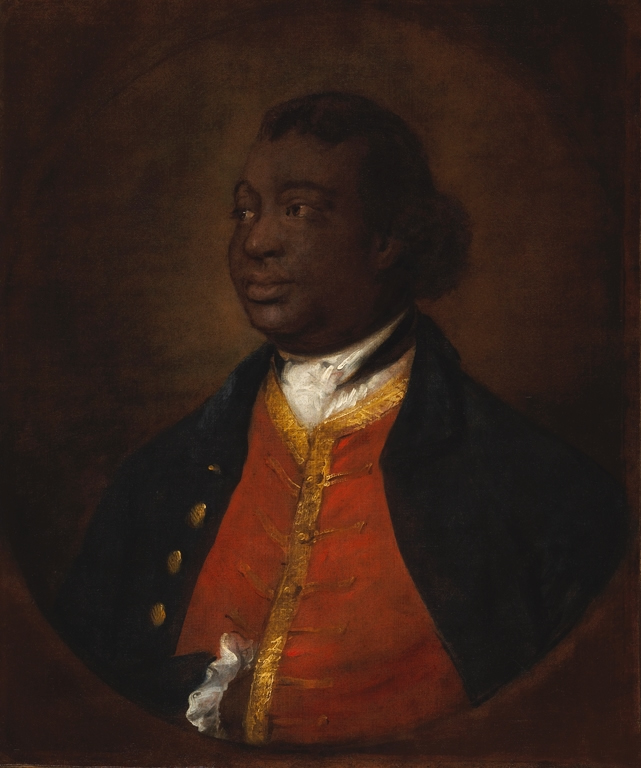
\includegraphics[scale=0.1]{chapters/img/Ignatius_Sancho,_1768.jpg}
%    \caption{Ignatius Sancho, 1768 by Thomas Gainsborough.}
%    \label{fig:LME_Sancho}
%\end{wrapfigure}
%took this out Dec 2021 because I couldn't get it to fit on the page in a sensible way


\end{texts}

\begin{texts}{Letter by Ignatius Sancho}
The Late Modern English period is the earliest period for which we have a significant number of English texts written by people of colour. Ignatius Sancho\ia{Sancho, Ignatius} was a Black writer, composer and slavery\is{slavery} survivor living in Britain during the eighteenth century. The letter below was written in July 1776 and addressed to a Mr. Sterne.\footnote{The text provided here was taken from the \emph{Emerging Voices} \glossterm{gl-corpus}{corpus}\is{corpora} \citep{Walkden2019}, and is originally from the 1784 edition available at \url{https://archive.org/details/lettersoflateign00sanc_0/}, pp. 89--91.}

\begin{quote}
    \internallinenumbers*{}
    REVEREND SIR,

    It would be an inſult to your humanity (or perhaps look like it) to aplogize for the liberty I am taking. -- I am one of thoſe people whom the vulgar and illiberal call ``Negurs.'' -- The firſt part of my life was rather unlucky, as I was placed in a family who judged ignorance the beſt and only ſecurity for obedience. -- A little reading and writing I got by unwearied application. -- The latter part of my life has been -- through God's bleſſing, truly fortunate, having ſpent it in the ſervice of the beſt families in the kingdom. -- My chief pleaſure has been books. -- Philanthropy I adore. -- How very much, good Sir, am I (amongſt millions) indebted to you for the character of your amiable uncle Toby! -- I declare, I would walk ten miles in the dog-days, to ſhake hands with the honeſt corporal. -- Your Sermons have touched me to the heart, and I hope have amended it, which brings me to the point. -- In your tenth diſcourſe, page ſeventy-eight, in the ſecond volume -- is this very affecting paſſage: -- ``Conſider how great a part of our ſpecies -- in all ages down to this -- have been trod under the feet of cruel and capricious tyrants, who would neither hear their cries, nor pity their diſtreſſes. -- Conſider ſlavery -- what it is -- how bitter a draught -- and how many millions are made to drink it!'' -- Of all my favourite authors not one has drawn a tear in favour of my miſerable black brethren -- excepting yourſelf, and the humane author of Sir George Elliſon. -- I think you will forgive me; -- I am ſure you will applaud me for beſeeching you to give one half-hour's attention to ſlavery, as it is at this day practiſed in our Weſt Indies. -- That ſubject, handled in your ſtriking manner, would eaſe the yoke (perhaps) of many; -- but if only of one -- Gracious God! -- what a feaſt to a benevolent heart! -- and, ſure I am, you are an Epicurean in acts of charity. -- You, who are univerſally read, and as univerſally admired -- you could not fail. -- Dear Sir, think in me you behold the uplifted hands of thouſands of my brother Moors. -- Grief (you pathetically obſerve) is eloquent; -- figure to yourſelf their attitudes; -- hear their ſupplicating addreſſes! -- Alas! -- you cannot refuſe. -- Humanity muſt comply -- in which hope I beg permiſſion to ſubſcribe myſelf,

    Reverend Sir, \&c.

    IGN. SANCHO.
%     \end{linenumbers}
\end{quote}
\end{texts}
\begin{furtherreading}
For a more in-depth discussion of Late Modern English, we recommend \citet{Beal2004} as an overall read with rich sociolinguistic discussions.\is{sociolinguistics} \citeauthor{Mugglestone2003}'s \citeyearpar{Mugglestone2003} \textit{Talking proper: the rise of accent as a social symbol} is another good read we strongly recommend, especially if you are interested in the history of \glossterm{gl-RP}{Received Pronunciation}.\il{English, Received Pronunciation} On prescriptivism\is{prescriptivism} and its effects, take a look at \textit{Fixing English} by Anne \citet{Curzan2014}.

For the history of American English,\il{English, American} with a focus on the rise of some of its distinct varieties, we recommend Chapter 6 in \citet{WolframSchilling-Estes2015}. For the linguistic situation in America vis-\`{a}-vis the War of Independence, we refer the readers to \citet{Martin2019}, with book section titles suggesting a thrilling read indeed (Part one: Noah Webster's\ia{Webster, Noah} battles; Part two: The Merriams at war). 

If you're interested in monographs focusing on other specific varieties of English\is{regional variation} (and their histories, to a variable extent), we refer you to \citet{Fritz2005} for Australian English,\il{English, Australian} \citet{Orkin2015} for Canadian English,\il{English, Canadian} \citet{Fought2003} for Chicano English,\il{English, Chicano} \citet{LukeRichards1982} and \citet{Edwards2015} for Hong Kong English,\il{English, Hong Kong} \citet{Hickey2007} for Irish English,\il{English, Irish} \citet{Gordonetal2004} for New Zealand English,\il{English, New Zealand} \citet{Leimgruber2013} for Singapore English,\il{English, Singapore} \citet{LanhamMacdonald1985} and \citet{Lass2002} -- and other contributions in \citet{Mesthrie2002} -- for South African English,\il{English, South African} \citet{Mesthrie1992} for South African Indian English,\il{English, South African Indian} and \citet{CouplandThomas1990} for Welsh English\il{English, Welsh} (Chapters 1, 2, 6, and 14 in particular). Volumes 5 and 6 of \textit{The Cambridge History of the English Language} (\citealp{Burchfield1994} and \citealp{Algeo2001}) offer contributions on English in Scotland,\il{English, Scottish} English in Wales, English in Ireland, English in Australia, English in the Caribbean,\il{English, Caribbean} English in New Zealand, English in South Africa, English in South Asia,\il{English, South Asian} and English in North America. And for \ili{Scots}, see \citet{Jones1997}.

(And if you are, like us, enchanted with the history of the progressive,\is{progressive} we recommend \citealp{Kranich2010}.)
\end{furtherreading}
